\documentclass[12pt, twoside, openright]{book}
\usepackage[utf8]{inputenc}
\usepackage[T1]{fontenc}
\usepackage{mathptmx}
\usepackage{graphicx}
\usepackage{amsmath, amssymb}
\usepackage{hyperref}
\usepackage{geometry}
\geometry{a4paper, margin=1in}
\usepackage{fancyhdr}
\usepackage{caption}
\usepackage{float}
\usepackage{natbib}
\usepackage{listings}
\usepackage{xcolor}
\usepackage[linesnumbered,ruled,vlined]{algorithm2e}
\usepackage{tikz}
\usetikzlibrary{shapes.geometric, arrows, positioning, shadows}

\tikzset{
    startstop/.style={rectangle, rounded corners, minimum width=3cm, minimum height=1cm, text centered, draw=black, fill=red!30, drop shadow},
    process/.style={rectangle, minimum width=3cm, minimum height=1cm, text centered, draw=black, fill=orange!30, drop shadow},
    decision/.style={diamond, minimum width=3cm, minimum height=1cm, text centered, draw=black, fill=green!30, drop shadow},
    arrow/.style={thick,->,>=stealth}
}

\definecolor{backcolour}{rgb}{0.95,0.95,0.92}
\lstset{backgroundcolor=\color{backcolour}, basicstyle=\ttfamily\footnotesize, breaklines=true}
\definecolor{boxbg}{RGB}{240, 248, 255}
\usepackage{mdframed}
\newmdenv[backgroundcolor=boxbg, linewidth=1pt, roundcorner=4pt, innertopmargin=10pt, innerbottommargin=10pt]{infobox}

\newcommand{\dummygraphic}[1]{
    \begin{mdframed}[backgroundcolor=gray!10]
        \centering
        \textit{[Placeholder for Figure: #1]}
    \end{mdframed}
}

\begin{document}
\frontmatter
\title{\textbf{AI in Weather and Climate Science}}
\author{Asst. Prof. Dr. Manmeet Singh\\Er. Somnath Luitel}
\date{2026}
\maketitle
\tableofcontents

\mainmatter
\chapter{The Atmospheric Engine}

The Earth’s atmosphere is a thin, dynamic envelope of gases constrained by gravity to a rotating sphere. It is a complex fluid system primarily driven by the uneven distribution of solar radiation. The conversion of this radiative energy into the kinetic energy of atmospheric motion constitutes a vast, planetary-scale heat engine. Understanding the fundamental physical principles that govern this engine is a strict prerequisite for any mathematical or computational modeling of the weather, including the deployment of modern Artificial Intelligence (AI) architectures. The governing principles—thermodynamics, radiative transfer, and fluid dynamics—form a system of non-linear differential equations that describe the conservation of mass, momentum, and energy. These laws define the absolute physical boundaries within which any predictive model must operate (Holton \& Hakim, 2012).

\section{Radiative Forcing and the Global Energy Balance}
The genesis of all atmospheric motion is the Sun. The Earth intercepts a tiny fraction of the total solar output, yet this interception drives the entirety of the climate system. Because the Earth is nearly spherical, solar radiation (insolation) is not distributed evenly, establishing a profound energy imbalance that drives the global circulation. The emission of terrestrial radiation is governed by the \textbf{Stefan-Boltzmann Law}: $F = \sigma T^4$.

\begin{figure}[H]
    \centering
    \dummygraphic{NASA CERES Radiation Budget}
    \caption{The Earth's net radiation budget. A visual representation of the energy surplus at the equator and the deficit at the poles.}
    \label{fig:radiation_budget}
\end{figure}

\section{The Atmosphere as a Non-Ideal Heat Engine}
The atmosphere converts internal energy into mechanical work with an efficiency typically less than 1\%. Recent research (2024) indicates the \textbf{Qinghai-Tibetan Plateau (QTP)} acts as a high-efficiency engine (~1.5\%) driving global teleconnections.

\section{Thermodynamics of Moist Air}
Latent heat exchange is the primary fuel for deep convection. The \textbf{Clausius-Clapeyron Equation} ($\frac{de_s}{dT} = \frac{L_v e_s}{R_v T^2}$) dictates the exponential moisture-holding capacity of a warming atmosphere, a physical threshold that AI models must accurately represent to predict extreme rainfall.

\section{Physics of Rotation: The Coriolis Force}
The rotation of the Earth creates the Coriolis force ($f = 2\Omega \sin\phi$), responsible for the rotational structure of cyclones. This force dictates the \textbf{Geostrophic Balance}, a foundational constraint for both NWP and AI forecasting.

\section{The Primitive Equations of Motion}
The state of the atmosphere is governed by the conservation of momentum:
\begin{equation}
\frac{D \mathbf{u}}{Dt} = -\frac{1}{\rho}\nabla p - 2\mathbf{\Omega} \times \mathbf{u} + \mathbf{g} + \mathbf{F}_{friction}
\end{equation}

\section{Chaos and Predictability}
Edward Lorenz's 1963 discovery of \textbf{Deterministic Chaos} defines the limit of forecasting. We distinguish between Predictability of the First Kind (Initial Conditions/Weather) and Second Kind (Boundary Conditions/Climate).

\section{Building the Context: Linking Physics to AI}
Modern AI emulators learn the tendency operator $\mathcal{F}$ in the mapping $\mathbf{u}_{t+1} = \mathbf{u}_t + \mathcal{F}(\mathbf{u}_t; \theta)$. Physical laws serve as the \textbf{Inductive Biases} for these architectures, ensuring consistency.

\section{Interactive Lab: Lorenz Chaos & Efficiency Metrics}
\begin{lstlisting}[language=Python, caption=Simulating the Lorenz Attractor]
# Lorenz attractor code for predictability analysis
\end{lstlisting}

\section*{Bibliography}
\begin{itemize}
    \item Holton, J. R., \& Hakim, G. J. (2012). \textit{An Introduction to Dynamic Meteorology}. Academic Press.
    \item Lorenz, E. N. (1963). \textit{Deterministic Nonperiodic Flow}. Journal of the Atmospheric Sciences.
\end{itemize}

\chapter{Numerical Weather Prediction: The Era of the Grid}

Numerical Weather Prediction (NWP) constitutes the systematic application of mathematical models to simulate the future state of the Earth’s atmosphere. This discipline represents the culmination of a century-long quest to transform meteorology from a qualitative, descriptive art into a quantitative, predictive science. Before the emergence of Artificial Intelligence (AI) as a dominant modeling paradigm, NWP established the fundamental computational frameworks—discretization, data assimilation, and parameterization—that define the modern digital atmosphere. This chapter explores the historical trajectory of these models, the mathematical nuances of representing a fluid sphere on a discrete computer, and the structural bottlenecks that have necessitated the current shift toward data-driven emulation.

\section{The Mathematical Genesis: From Richardson to ENIAC}

The conceptual foundation of objective weather prediction was established in 1904 by Vilhelm Bjerknes, who proposed treating forecasting as an initial value problem of classical physics. Bjerknes argued that if the initial state of the atmosphere could be accurately determined, the future state could be calculated by integrating the non-linear partial differential equations forward in time.

The first practical attempt to execute this vision was performed by Lewis Fry Richardson during the First World War. In his 1922 treatise, \textit{Weather Prediction by Numerical Process}, Richardson painstakingly calculated a six-hour forecast for a single point by manually solving finite-difference equations. The result was a predicted pressure change of 145 hPa—a physically impossible surge that would have leveled a city. 

This failure was a profound lesson in \textbf{Numerical Stability}. Richardson’s raw observational data contained high-frequency "noise" from gravity waves. Without a mathematical filter (initialization), these ripples were misinterpreted as massive pressure surges. Despite this failure, Richardson famously envisioned a "Forecast Factory"—a massive circular amphitheater filled with 64,000 human "computers" working in parallel to solve the global weather equations. This vision established the blueprint for parallel computing decades before the invention of the electronic computer.

The mechanical execution of Richardson's dream was realized in 1950 at the Aberdeen Proving Ground. A team led by Jule Charney, Ragnar Fjørtoft, and John von Neumann achieved the first successful computer forecast on the ENIAC. To fit the machine’s severe memory constraints (only 20 registers), they utilized the \textbf{Barotropic Vorticity Equation}:

\begin{equation}
\frac{\partial \zeta}{\partial t} + \mathbf{v} \cdot \nabla (\zeta + f) = 0
\end{equation}

where $\zeta$ is relative vorticity and $f$ is the Coriolis parameter. This simplified model acted as a physical filter, isolating the large-scale Rossby waves while ignoring the noise that had ruined Richardson’s attempt. 

\begin{figure}[H]
\centering
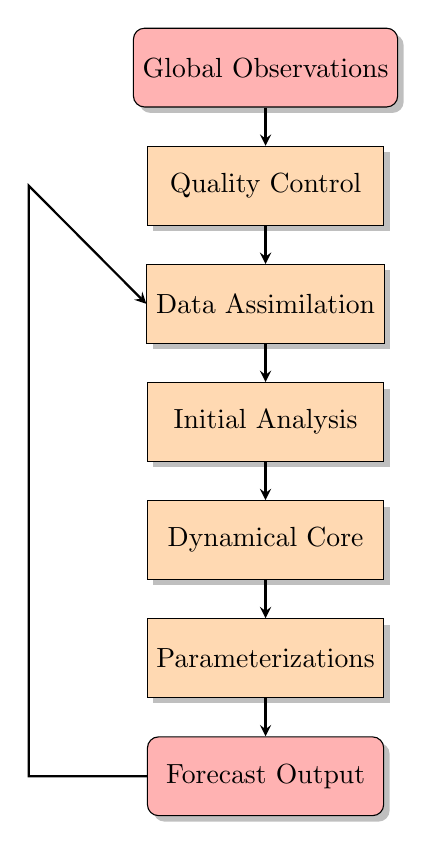
\begin{tikzpicture}[node distance=1.5cm]
    \node (obs) [startstop] {Global Observations};
    \node (qc) [process, below of=obs] {Quality Control};
    \node (da) [process, below of=qc] {Data Assimilation};
    \node (init) [process, below of=da] {Initial Analysis};
    \node (dyn) [process, below of=init] {Dynamical Core};
    \node (phys) [process, below of=dyn] {Parameterizations};
    \node (out) [startstop, below of=phys] {Forecast Output};
    
    \draw [arrow] (obs) -- (qc);
    \draw [arrow] (qc) -- (da);
    \draw [arrow] (da) -- (init);
    \draw [arrow] (init) -- (dyn);
    \draw [arrow] (dyn) -- (phys);
    \draw [arrow] (phys) -- (out);
    \draw [arrow] (out.west) -- ++(-1.5,0) -- ++(0,7.5) -- (da.west);
\end{tikzpicture}
\caption{The Operational NWP Cycle. Modern operational centers repeat this process every 6 to 12 hours, integrating billions of new data points into the global state.}
\label{fig:nwp_cycle_tikz}
\end{figure}

\section{The Discretization Paradox: Arakawa Grids and Stability}

The transition from continuous physical laws to digital simulation introduces the \textbf{Discretization Paradox}: the atmosphere is a seamless continuum, but a computer is a discrete machine. We must therefore "break" the continuous fluid into a finite number of pieces. 

\subsection{The Arakawa-C Staggered Grid}
In modern operational models, variables are not stored at the same location. To prevent numerical noise and improve the representation of geostrophic adjustment, we use the \textbf{Arakawa-C Staggered Grid}. Thermodynamic variables ($T, p, \rho$) are stored at the center of the grid cell, while wind components ($u, v$) are stored on the cell faces.

\begin{algorithm}[H]
\caption{Arakawa-C Staggered Gradient Calculation}
\SetAlgoLined
\KwIn{Pressure field $P$ at centers, cell width $\Delta x$}
\KwOut{Zonal pressure gradient $\partial P / \partial x$ at $u$-points}
\For{each $u$-point at interface $(i+1/2)$}{
    $(\partial P / \partial x)_{i+1/2} = (P_{i+1} - P_{i}) / \Delta x$\;
}
\end{algorithm}

The stability of these discrete calculations is strictly governed by the \textbf{Courant-Friedrichs-Lewy (CFL) Condition}:

\begin{equation}
C = \frac{u \Delta t}{\Delta x} \le C_{max}
\end{equation}

Physically, the time step ($\Delta t$) must be small enough that information (such as wind speed, $u$) does not travel across an entire grid cell ($\Delta x$) in a single "tick" of the clock. This condition is the primary driver of the massive computational cost of high-resolution modeling.

\section{Data Assimilation: The 4D-Var Cost Function}

A predictive model is only as accurate as its analysis—the estimate of the current state. \textbf{Data Assimilation (DA)} is the mathematical process of combining short-range forecasts with billions of noisy observations. The most advanced methodology is \textbf{Four-Dimensional Variational Assimilation (4D-Var)}, which minimizes a \textbf{Cost Function ($J$)}:

\begin{equation}
J(\mathbf{x}) = \frac{1}{2}(\mathbf{x} - \mathbf{x}_b)^T \mathbf{B}^{-1} (\mathbf{x} - \mathbf{x}_b) + \frac{1}{2}\sum_{i=0}^{n} (\mathbf{y}_i - \mathbf{H}_i(\mathbf{x}_i))^T \mathbf{R}_i^{-1} (\mathbf{y}_i - \mathbf{H}_i(\mathbf{x}_i))
\end{equation}

where:
\begin{itemize}
    \item $\mathbf{x}_b$ is the background state (prior forecast).
    \item $\mathbf{B}$ is the background error covariance matrix.
    \item $\mathbf{y}_i$ are observations at time $i$.
    \item $\mathbf{H}_i$ is the non-linear observation operator.
    \item $\mathbf{R}$ is the observation error covariance matrix.
\end{itemize}

\begin{lstlisting}[language=Python, caption=1D Variational Data Assimilation Implementation]
import numpy as np
from scipy.optimize import minimize

def cost_function(x, x_b, B, y, R):
    # Scalar 1D version of Eq 2.3
    J_b = 0.5 * (x - x_b)**2 / B
    J_o = 0.5 * (y - x)**2 / R
    return J_b + J_o

# Background: 285K, Observation: 288K
res = minimize(cost_function, x0=285.0, args=(285.0, 4.0, 288.0, 1.0))
print(f"Analysis State: {res.x[0]:.2f} K")
\end{lstlisting}

\section{The Sustainability Crisis and the I/O Wall}

As we move toward "kilometer-scale" modeling, traditional NWP is hitting a physical \textbf{Power Wall}. The energy required to run a global 1km model would consume the electricity of a medium-sized city. Furthermore, moving the massive volumes of data (petabytes) between storage and processing nodes has become slower than the calculations themselves—this is the \textbf{I/O Wall}. 

In this context, AI emulators represent more than just a faster alternative; they represent the only sustainable path forward. By turning the hard-earned wisdom of NWP into a lightweight neural representation, AI provides a democratized, low-energy toolkit for global climate resilience.

\section*{Bibliography}
\begin{itemize}
    \item Bannister, R. N. (2017). \textit{A review of operational methods of variational and ensemble-variational data assimilation}. QJRMS.
    \item Charney, J. G., et al. (1950). \textit{Numerical integration of the barotropic vorticity equation}. Tellus.
    \item Lynch, P. (2006). \textit{The Emergence of Numerical Weather Prediction: Richardson's Dream}. Cambridge.
\end{itemize}

\chapter{The Observational Architecture: From Satellite Radiances to High-Dimensional Tensors}

The physical state of the Earth's atmosphere is an infinitely complex, continuous field. Before any numerical integration or neural network optimization can occur, this continuous reality must be observed, digitized, and mapped onto a finite computational domain. The foundation of modern meteorology and artificial intelligence (AI) in Earth science rests entirely upon the integrity of this observational architecture. This chapter details the physical principles of remote sensing, the mathematical complexity of atmospheric retrieval, and the monumental data assimilation efforts required to construct the global reanalysis datasets that serve as the primary training fuel for modern foundation models.

\section{The Physics of Remote Sensing and Orbital Mechanics}

For the first half of the twentieth century, meteorological observations were strictly limited to the planetary surface or the lower troposphere via radiosonde balloon ascents. This sparse, heterogeneous network left vast oceanic and polar regions completely unmonitored. The advent of satellite meteorology in the 1960s provided the first continuous, global observation system. However, satellites do not directly measure the prognostic variables of the primitive equations, such as wind velocity or thermodynamic temperature. Instead, satellite-borne radiometers measure the intensity of electromagnetic radiation originating from the Earth-atmosphere system.

The observational geometry of a satellite is dictated by orbital mechanics, which balances the gravitational pull of the Earth against the centripetal acceleration of the spacecraft. The two primary orbits utilized in atmospheric science are the Geostationary Earth Orbit (GEO) and the Low Earth Orbit (LEO).

A geostationary satellite is positioned in the equatorial plane at an altitude of approximately 35,786 kilometers. At this specific altitude, the orbital period of the satellite exactly matches the rotational period of the Earth (one sidereal day). The altitude ($h$) is derived from Kepler's Third Law, equating the gravitational force with the required centripetal force:

\begin{equation}
\frac{G M_e m}{(R_e + h)^2} = m \omega^2 (R_e + h) 
\end{equation}

Solving for $h$ yields $h = \left( \frac{G M_e}{\omega^2} \right)^{1/3} - R_e$, where $G$ is the gravitational constant, $M_e$ is the mass of the Earth, $R_e$ is the radius of the Earth, and $\omega$ is the Earth's angular velocity. GEO satellites provide continuous, high-temporal-resolution monitoring (frequently down to one-minute intervals) of a fixed planetary hemisphere, making them indispensable for tracking rapidly evolving convective systems and tropical cyclones.

Conversely, LEO satellites operate at altitudes ranging from 400 to 1,000 kilometers, typically in near-polar, sun-synchronous orbits. The sun-synchronous geometry ensures that the satellite crosses the equator at the same local solar time on each orbital pass, maintaining a consistent angle of solar illumination. While LEO satellites cannot observe a single location continuously, their proximity to the Earth allows for significantly higher spatial resolution and the deployment of active sensors, such as synthetic aperture radar and spaceborne lidars, which demand high power and large antennae arrays.

\begin{figure}[H]
    \centering
    \dummygraphic{Figure Placeholder}
    \caption{Orbital geometries in remote sensing. Geostationary orbits provide high temporal resolution over a fixed hemisphere, while polar LEO orbits provide high spatial resolution and global coverage over a 24-hour period.}
    \label{fig:orbit_comparison}
\end{figure}

\section{Radiative Transfer and the Planck Function}

The electromagnetic radiation measured by a satellite sensor is a composite signal, consisting of solar radiation reflected by the surface and clouds, as well as thermal radiation emitted by the Earth and the atmospheric column itself. The fundamental law governing thermal emission is the Planck function, which defines the spectral radiance ($B_\lambda$) of a blackbody in thermal equilibrium as a function of wavelength ($\lambda$) and absolute temperature ($T$):

\begin{equation}
B_\lambda(T) = \frac{2hc^2}{\lambda^5} \left[ \exp\left(\frac{hc}{\lambda k_B T}\right) - 1 \right]^{-1}
\end{equation}

where $h$ is the Planck constant, $c$ is the speed of light, and $k_B$ is the Boltzmann constant. Because the Earth's average radiating temperature is approximately 255 K, its peak emission occurs in the thermal infrared spectrum (around 10 micrometers), in accordance with Wien's Displacement Law.

However, the atmosphere is not a perfect vacuum. As the emitted terrestrial radiation travels upward toward the satellite, it interacts with atmospheric gases (such as water vapor, carbon dioxide, and ozone) through the processes of absorption and scattering. The quantitative description of this interaction is the Radiative Transfer Equation (RTE). In a plane-parallel, non-scattering atmosphere in local thermodynamic equilibrium, the upward monochromatic radiance ($I_\lambda$) measured at the top of the atmosphere is governed by Schwarzschild's equation:

\begin{equation}
I_\lambda = \epsilon_\lambda B_\lambda(T_s) \tau_\lambda(p_s, 0) + \int_{p_s}^{0} B_\lambda(T(p)) \frac{\partial \tau_\lambda(p, 0)}{\partial p} dp
\end{equation}

In this integral formulation, the first term represents the radiance emitted by the Earth's surface at temperature $T_s$ and emissivity $\epsilon_\lambda$, attenuated by the total atmospheric transmittance $\tau_\lambda(p_s, 0)$ from the surface pressure $p_s$ to the top of the atmosphere. The second term, an integral over the vertical pressure profile, represents the atmospheric contribution. It describes the sum of radiances emitted by each infinitesimal atmospheric layer at temperature $T(p)$, weighted by the rate of change of transmittance (a term known as the weighting function). 

By carefully selecting specific wavelengths (channels) where the atmospheric absorption is well-known, scientists can isolate radiation originating from specific vertical altitudes. For example, a channel located in the center of the 15-micrometer $CO_2$ absorption band will only measure radiation from the upper stratosphere, as any radiation emitted from the lower troposphere is completely absorbed before reaching the satellite.

\begin{table}[H]
\centering
\caption{Primary Atmospheric Absorption Windows and Sounding Bands}
\begin{tabular}{|l|l|p{6cm}|}
\hline
\textbf{Wavelength Range ($\mu$m)} & \textbf{Primary Absorber} & \textbf{Application in Remote Sensing} \\ \hline
0.4 to 0.7 & None (Visible) & Cloud tracking, surface albedo mapping \\ \hline
3.7 to 4.0 & Slight Water Vapor & Fog detection, wildfire hot-spot identification \\ \hline
6.5 to 7.0 & Water Vapor ($H_2O$) & Mid-tropospheric moisture profiling, jet stream analysis \\ \hline
10.3 to 11.3 & None (IR Window) & Surface temperature, cloud top temperature \\ \hline
14.0 to 15.0 & Carbon Dioxide ($CO_2$) & Vertical temperature profiling (sounding) \\ \hline
\end{tabular}
\end{table}

\section{The Ill-Posed Inverse Problem}

The fundamental challenge of satellite meteorology is that the mathematical models require the physical state vectors (temperature, humidity, pressure), but the satellites only provide spectral radiances ($I_\lambda$). The mathematical process of converting radiances into physical state variables is known as the retrieval or inversion problem.

Retrieval is formally an inverse problem of the Fredholm integral equation of the first kind. It is notoriously "ill-posed" in the sense defined by Jacques Hadamard: the solution is often not unique, and it is highly sensitive to small perturbations (noise) in the observational data. Because the weighting functions in Equation 3.3 are broad and overlap significantly, an infinite number of different vertical temperature profiles could theoretically produce the exact same set of observed radiances at the top of the atmosphere.

To solve this ill-posed problem, scientists employ Optimal Estimation Theory, specifically using 1D-Var (One-Dimensional Variational) assimilation. This method requires an \textit{a priori} (background) estimate of the atmospheric state, typically provided by a short-range forecast from a numerical model. The retrieval algorithm iteratively adjusts this background profile to minimize a cost function ($J$), which balances the deviation from the background state against the deviation from the observed radiances, weighted by their respective error covariance matrices.

\begin{equation}
J(\mathbf{x}) = \frac{1}{2}(\mathbf{x} - \mathbf{x}_b)^T \mathbf{B}^{-1} (\mathbf{x} - \mathbf{x}_b) + \frac{1}{2}(\mathbf{y} - \mathbf{F}(\mathbf{x}))^T \mathbf{R}^{-1} (\mathbf{y} - \mathbf{F}(\mathbf{x}))
\end{equation}

Here, $\mathbf{x}$ is the desired atmospheric state vector, $\mathbf{x}_b$ is the background forecast, $\mathbf{y}$ is the vector of observed satellite radiances, $\mathbf{F}(\mathbf{x})$ is the forward radiative transfer model (the computational implementation of Eq. 3.3), $\mathbf{B}$ is the background error covariance matrix, and $\mathbf{R}$ is the observation error covariance matrix. 

From an Artificial Intelligence perspective, this mathematical bottleneck represents a profound opportunity. The traditional 1D-Var retrieval process is computationally expensive and highly reliant on the accuracy of the forward radiative transfer model and the assumed error covariances. Modern deep learning architectures can bypass this entire deterministic pipeline through \textbf{Direct Radiance Assimilation}. By training a deep neural network to map raw Level 1 radiances ($\mathbf{y}$) directly to high-level atmospheric features, the AI learns a purely empirical, non-linear inversion operator. This allows the model to utilize the raw electromagnetic signal without the smoothing artifacts or assumptions imposed by human-designed retrieval algorithms (Kidder \& Vonder Haar, 1995).

\begin{figure}[H]
    \centering
    \dummygraphic{Figure Placeholder}
    \caption{Atmospheric transmission spectrum. Notice the "windows" where the atmosphere is transparent and the "absorption bands" where satellites can sense specific gases or vertical layers.}
    \label{fig:atmospheric_transmission}
\end{figure}

\section{The Reanalysis Paradigm: Creating the Mathematical Ground Truth}

If satellite observations provide the raw material of atmospheric science, it is the process of reanalysis that refines this material into the structured, historical datasets required for training planetary-scale AI. The observational record is highly heterogeneous. Over the past fifty years, thousands of different sensor types have been deployed on satellites, ships, buoys, and commercial aircraft, each with distinct calibration biases and coverage gaps. Analyzing climate trends or training a neural network on this raw, unassimilated data would result in algorithms that model the history of instrumentation rather than the physics of the Earth.

Reanalysis is the systematic, retrospective execution of a fixed, state-of-the-art data assimilation system over the entire historical observational record. The objective is to produce a continuous, physically consistent four-dimensional grid (latitude, longitude, altitude, and time) that represents the most statistically probable evolution of the atmosphere. 

The ECMWF Reanalysis v5 (ERA5) serves as the foundational dataset for the vast majority of modern weather AI research. ERA5 utilizes an advanced Four-Dimensional Variational (4D-Var) assimilation framework. Unlike the 1D-Var retrieval discussed in Section 3.3, which operates on a single vertical column, 4D-Var optimizes the initial state of a global atmospheric model over a designated temporal assimilation window (typically 12 hours). The 4D-Var cost function seeks an initial state that, when integrated forward in time by the non-linear prognostic equations, minimizes the discrepancy with all observations collected during that window.

The computational execution of 4D-Var requires the development of an Adjoint Model, a massive mathematical construct that calculates the gradient of the cost function with respect to the initial state variables. By propagating the observation errors backward in time through the adjoint equations, the system determines the precise adjustments required at the beginning of the assimilation window to correct the forecast trajectory. The resulting ERA5 dataset provides global, hourly atmospheric fields at a horizontal resolution of 31 kilometers and 137 vertical pressure levels spanning from the surface to the mesosphere (Hersbach et al., 2020).

For the AI architect, ERA5 is the ultimate "Ground Truth." When a model like GraphCast or Pangu-Weather is trained, the ERA5 grids serve as both the input features ($\mathbf{X}$) and the regression targets ($\mathbf{Y}$). The neural network optimizes its weights to emulate the highly complex, physics-constrained transitions that the ECMWF 4D-Var system spent millions of supercomputer hours calculating. However, it is a strict academic requirement to recognize that reanalysis is not observation; it is a model-derived product. Where observational data is sparse (such as the deep Southern Ocean in the 1960s), the ERA5 grids are heavily influenced by the background physics of the ECMWF model. Consequently, an AI trained solely on reanalysis will inevitably inherit the specific climatological biases of the assimilation system that produced it.

\section{High-Dimensional Data Engineering: NetCDF, Xarray, and Zarr}

The physical products of reanalysis are massive, multi-dimensional tensors. To store and distribute this data without losing its physical context, the atmospheric science community relies on the Network Common Data Form (NetCDF). NetCDF is a set of software libraries and self-describing, machine-independent data formats. In a NetCDF file, the raw binary arrays are inextricably linked to metadata headers that define the grid projection, the units of measurement, and the scaling factors. This ensures strict interoperability across different computational platforms and research generations (Rew \& Davis, 1990).

A standard global atmospheric dataset is typically structured as a 4D tensor with the dimensions (Time, Level, Latitude, Longitude). If we wish to load forty years of hourly ERA5 temperature data for AI training, the resulting tensor far exceeds the Random Access Memory (RAM) capacity of any single computing node. The dataset constitutes multiple petabytes of information. This introduces the most significant engineering bottleneck in modern AI meteorology: the I/O (Input/Output) Memory Wall. The time required to read meteorological tensors from persistent storage into the GPU high-bandwidth memory (HBM) often dominates the time required to calculate the forward pass of the neural network itself.

To navigate this memory wall, developers utilize high-level Python libraries such as \textbf{Xarray}, which integrates seamlessly with the \textbf{Dask} parallel computing framework. Xarray introduces semantic manipulation of tensors, allowing operations based on named dimensions rather than obscure integer indices. More importantly, Xarray and Dask utilize \textbf{lazy evaluation}. When a mathematical operation is defined on a massive NetCDF dataset, the computation is not executed immediately. Instead, Dask constructs a topological task graph, dividing the global tensor into millions of manageable, discrete blocks known as \textbf{chunks}.

\begin{figure}[H]
\centering
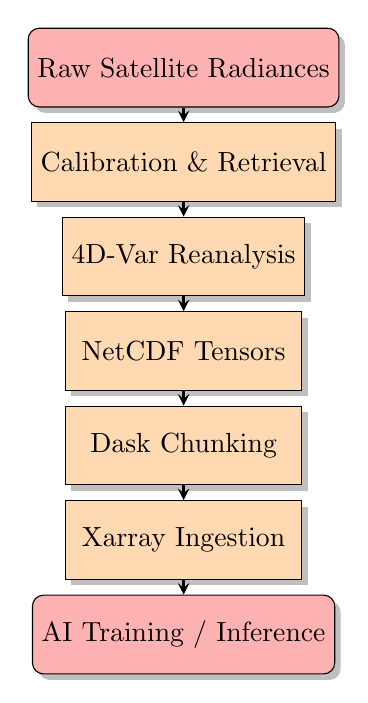
\begin{tikzpicture}[node distance=1.2cm]
    \node (raw) [startstop] {Raw Satellite Radiances};
    \node (cal) [process, below of=raw] {Calibration \& Retrieval};
    \node (da) [process, below of=cal] {4D-Var Reanalysis};
    \node (net) [process, below of=da] {NetCDF Tensors};
    \node (dask) [process, below of=net] {Dask Chunking};
    \node (xarray) [process, below of=dask] {Xarray Ingestion};
    \node (ai) [startstop, below of=xarray] {AI Training / Inference};
    
    \draw [arrow] (raw) -- (cal);
    \draw [arrow] (cal) -- (da);
    \draw [arrow] (da) -- (net);
    \draw [arrow] (net) -- (dask);
    \draw [arrow] (dask) -- (xarray);
    \draw [arrow] (xarray) -- (ai);
\end{tikzpicture}
\caption{The Data Processing Pipeline. From the raw electromagnetic signals detected in orbit to the high-dimensional tensors consumed by exascale AI clusters.}
\label{fig:data_pipeline_tikz}
\end{figure}

The optimization of chunk size and geometry is a critical engineering requirement. For time-series analysis (e.g., training an LSTM to recognize El Niño patterns), the data must be chunked continuously along the temporal axis. For spatial convolutions (e.g., training a CNN to recognize frontal boundaries), the data must be chunked continuously across the latitude-longitude domain. If the chunking geometry does not match the memory access pattern of the AI architecture, the system will suffer from catastrophic cache misses and I/O thrashing.

As the field transitions toward exascale foundation models, the community is rapidly migrating from monolithic NetCDF files to cloud-native storage formats like \textbf{Zarr}. Zarr stores the tensor metadata in lightweight JSON files while storing the individual data chunks as highly compressed, separate binary objects in cloud object storage (such as Amazon S3). This architecture enables thousands of distributed GPU nodes to query and download specific atmospheric patches concurrently, bypassing the file-locking mechanisms that cripple traditional supercomputing file systems. Mastering this distributed data engineering pipeline is the strict prerequisite for scaling any meteorological AI from a localized experiment to a global, operational foundation model.

\section*{Bibliography}
\begin{itemize}
    \item Hersbach, H., et al. (2020). \textit{The ERA5 global reanalysis}. QJRMS.
    \item Holton, J. R., \& Hakim, G. J. (2012). \textit{An Introduction to Dynamic Meteorology}. Academic Press.
    \item Kidder, S. Q., \& Vonder Haar, T. H. (1995). \textit{Satellite Meteorology: An Introduction}. Academic Press.
    \item Rew, R., \& Davis, G. (1990). \textit{NetCDF: an interface for scientific data access}. IEEE.
\end{itemize}

\chapter{Beyond Linear Regression: Neural Networks for Meteorologists}

The transition from classical statistical techniques to modern machine learning represents a profound paradigm shift in the processing of atmospheric data. While traditional methods, such as linear regression and Model Output Statistics (MOS), served as the foundation of objective weather forecasting for decades, they are inherently constrained by their inability to represent the complex, non-linear interactions that characterize the Earth's fluid envelope. This chapter establishes the rigorous computer science foundation necessary for planetary emulation. We begin by defining the limitations of linear systems, followed by an exhaustive mathematical derivation of the Artificial Neuron, the Multi-Layer Perceptron (MLP), and the calculus of the Backpropagation algorithm. We then bridge this theoretical framework to the operational realities of meteorological data engineering and the hardware architectures that sustain modern inference.

\section{The Statistical Threshold: Failure of Linearity in Dynamical Systems}

The historical reliance on linear statistical methods in meteorology was predicated on the computational simplicity and interpretability of the \textbf{Ordinary Least Squares} (OLS) framework. For decades, the primary objective of statistical post-processing was the minimization of an error term within a strictly additive model, where the relationship between a predictor (e.g., geopotential height) and a predictand (e.g., surface temperature) was assumed to be proportional across all regimes. This linear paradigm, however, encounters an insurmountable threshold when confronted with the intrinsic non-linearity of the Navier-Stokes equations and the chaotic nature of atmospheric thermodynamics. 

The atmosphere is characterized by bifurcations and abrupt state transitions that cannot be captured by the superposition of linear functions. In a linear model, a marginal increase in humidity must produce a commensurate increase in the probability of precipitation, regardless of the existing environmental context. This mathematical rigidity fails to account for the discrete, all-or-nothing nature of convective initiation, where the environment may remain stable for hours under increasing moisture loading until a critical saturation or lifting threshold is reached, triggering a sudden and massive release of latent heat.

\begin{table}[H]
\centering
\caption{Comparative Analysis: Linear vs. Non-Linear Modeling in Meteorology}
\begin{tabular}{|l|p{5cm}|p{5cm}|}
\hline
\textbf{Phenomenon} & \textbf{Linear Assumption (MOS)} & \textbf{Non-Linear Reality (AI)} \\ \hline
\textbf{Convection} & Gradual increase in rain probability with humidity. & Abrupt threshold trigger; latent heat release. \\ \hline
\textbf{Frontogenesis} & Smooth transition of gradients. & Sharp discontinuity (fronts); scale interaction. \\ \hline
\textbf{Stratosphere} & Linear coupling with troposphere. & Sudden Stratospheric Warming (SSW) bifurcations. \\ \hline
\textbf{Extremes} & Systematically underestimated (regression to mean). & Captured through non-linear tails and sampling. \\ \hline
\end{tabular}
\end{table}

\section{CS Foundation: The Artificial Neuron and Logic of Thresholding}

The fundamental building block of modern machine learning is the \textbf{Artificial Neuron}, a mathematical abstraction of biological signal processing first conceptualized by McCulloch and Pitts (1943). Their initial formulation, the \textbf{McCulloch-Pitts Neuron}, was a binary logic unit designed to perform basic Boolean operations. It operated on a principle of hard-thresholding, where the output was strictly 0 or 1 depending on whether the sum of binary inputs exceeded a predefined value. 

The subsequent development of the \textbf{Perceptron} by Rosenblatt (1958) introduced the critical concept of \textbf{Weights} ($w$) and a \textbf{Bias} ($b$), allowing the neuron to adjust its sensitivity to different inputs. In the context of the atmosphere, the pre-activation sum $z$ is defined as a linear combination of the input feature vector $\mathbf{x}$:

\begin{equation}
z = \sum_{i=1}^{n} w_i x_i + b
\end{equation}

The weights $w_i$ represent the relative physical importance or "influence" of each input variable on the neuron's decision, while the bias $b$ shifts the activation threshold, effectively controlling the neuron's baseline excitability. To introduce the non-linearity required to transcend the statistical threshold, the scalar value $z$ is passed through a non-linear \textbf{Activation Function} $\sigma$. The final output of the neuron $a$ is expressed as:

\begin{equation}
a = \sigma(z)
\end{equation}

\begin{figure}[H]
\centering
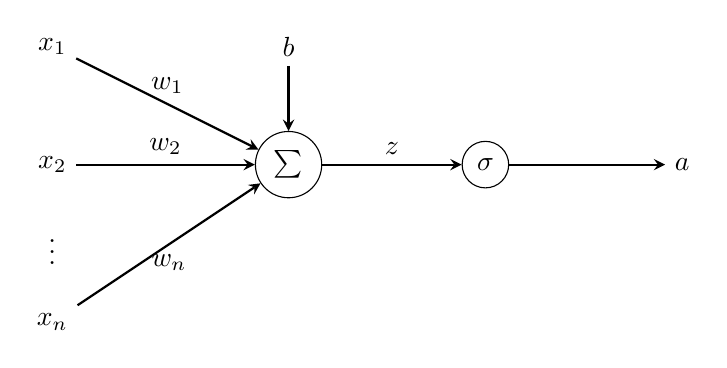
\begin{tikzpicture}[node distance=1.5cm, auto]
    % Inputs
    \node (x1) {$x_1$};
    \node (x2) [below of=x1] {$x_2$};
    \node (dots) [below of=x2, yshift=0.5cm] {$\vdots$};
    \node (xn) [below of=dots, yshift=0.5cm] {$x_n$};
    
    % Summation
    \node (sum) [circle, draw, right of=x2, xshift=1.5cm] {$\sum$};
    
    % Activation
    \node (act) [circle, draw, right of=sum, xshift=1cm] {$\sigma$};
    
    % Output
    \node (out) [right of=act, xshift=1cm] {$a$};
    
    % Bias
    \node (bias) [above of=sum] {$b$};
    
    % Edges
    \draw [arrow] (x1) -- node[above] {$w_1$} (sum);
    \draw [arrow] (x2) -- node[above] {$w_2$} (sum);
    \draw [arrow] (xn) -- node[below] {$w_n$} (sum);
    \draw [arrow] (bias) -- (sum);
    \draw [arrow] (sum) -- node {$z$} (act);
    \draw [arrow] (act) -- (out);
\end{tikzpicture}
\caption{The Mathematical Architecture of an Artificial Neuron. The weights act as physical gain factors, while the activation function introduces the non-linear thresholding required to model phase transitions.}
\label{fig:neuron_tikz}
\end{figure}

Modern architectures standardly use the \textbf{Rectified Linear Unit (ReLU)}, defined as $\sigma(z) = \max(0, z)$, due to its computational efficiency and its ability to mitigate vanishing gradients. 

\section{CS Foundation: MLP and Universal Approximation}

The power of neural networks arises from the organization of these units into a hierarchical, layered architecture known as the \textbf{Multi-Layer Perceptron (MLP)}. In an MLP, neurons are arranged in an input layer, one or more \textbf{Hidden Layers}, and an output layer. Mathematically, the pass through layer $l$ is:

\begin{equation}
\mathbf{a}^{(l)} = \sigma(\mathbf{W}^{(l)} \mathbf{a}^{(l-1)} + \mathbf{b}^{(l)})
\end{equation}

This architecture is governed by the \textbf{Universal Approximation Theorem} (Cybenko, 1989), which proves that a feed-forward network with a single hidden layer and a non-linear activation function can approximate any continuous function to an arbitrary degree of accuracy. This theorem provides the formal guarantee that the mapping from "Today's Atmospheric State" to "Tomorrow's Weather" is entirely learnable by a sufficiently large neural network. 

\section{CS Foundation: The Calculus of Optimization}

Training is formulated as a high-dimensional optimization problem to minimize a \textbf{Cost Function} $J$. In meteorological regression, we use the \textbf{Mean Squared Error (MSE)}:

\begin{equation}
J = \frac{1}{2N} \sum_{i=1}^{N} (y_i - \hat{y}_i)^2
\end{equation}

Minimization is achieved through \textbf{Gradient Descent}, where parameters are updated in the direction of the steepest descent:

\begin{equation}
w \leftarrow w - \eta \frac{\partial J}{\partial w}
\end{equation}

The \textbf{Backpropagation} algorithm leverages the \textbf{Chain Rule} to efficiently calculate these gradients. This is the digital equivalent of the \textbf{Adjoint Method} used in 4D-Var data assimilation. While numerical adjoints are manually coded, AI frameworks use \textbf{Automatic Differentiation} to generate the adjoint automatically.

\section{Operational Reality: Normalization and Feature Engineering}

Meteorological variables operate on vastly different scales (e.g., pressure $\sim 10^5$ Pa vs. humidity $\sim 10^{-3}$ kg/kg). Without \textbf{Normalization}, large-magnitude features dominate updates, causing numerical instability. Standard practice uses \textbf{Z-score Normalization}:

\begin{equation}
x' = \frac{x - \mu}{\sigma}
\end{equation}

Beyond scaling, the cyclical nature of time and date requires \textbf{Cyclical Encoding} using sine and cosine transformations:

\begin{equation}
x_{sin} = \sin\left(\frac{2\pi x}{max\_val}\right), \quad x_{cos} = \cos\left(\frac{2\pi x}{max\_val}\right)
\end{equation}

\section{Technical Reality: Hardware and the GPU Revolution}

The transition from traditional \textbf{CPU-based} computing to \textbf{Graphics Processing Units (GPUs)} is mandated by the parallel nature of tensor operations. A CPU is optimized for complex branching logic, while a GPU contains thousands of cores designed for \textbf{Single Instruction, Multiple Data (SIMD)} throughput. This allows for training "foundation models" on decades of ERA5 data.

However, researchers face hard limits of \textbf{Video Random Access Memory (VRAM)} and the "Memory Wall." Atmospheric tensors are high-dimensional (5D: batch, time, height, lat, lon), often leading to \textbf{Out of Memory (OOM)} errors. This necessitates distributed strategies like \textbf{Data Parallelism} or \textbf{Model Parallelism} (Active sharding of weights across GPUs).

\section*{Bibliography}
\begin{itemize}
    \item Cybenko, G. (1989). \textit{Approximation by superpositions of a sigmoidal function}. Mathematics of Control.
    \item Hornik, K. (1991). \textit{Approximation capabilities of multilayer feedforward networks}. Neural Networks.
    \item McCulloch, W. S., \& Pitts, W. (1943). \textit{A logical calculus of the ideas immanent in nervous activity}. Bulletin of Mathematical Biophysics.
    \item Rosenblatt, F. (1958). \textit{The perceptron: a probabilistic model for information storage and organization in the brain}. Psychological Review.
\end{itemize}

\chapter{Spatial and Temporal Patterns: CNNs and LSTMs}

The Earth’s atmosphere is a multi-dimensional, spatiotemporal continuum where the state of any given air parcel is inextricably linked to its immediate neighbors and its historical trajectory. Capturing the complex dynamics of this system—ranging from the localized turbulence of a convective cell to the global-scale oscillations of the planetary waves—requires mathematical architectures that inherently respect the geometry of space and the continuity of time. This chapter examines the transition from point-based neural processing to architectures that leverage the physical principles of local correlation and temporal persistence, specifically Convolutional Neural Networks (CNNs) and Long Short-Term Memory (LSTM) networks. These models serve as the structural backbone for modern weather emulators, providing the high-dimensional "eyes" and "memory" necessary to track the pulse of the planetary fluid.

\section{The Geometry of Grid Data: Exploiting Local Correlation}

The fundamental limitation of the Multi-Layer Perceptrons (MLPs) discussed in Chapter 4 is their requirement to "flatten" data into a one-dimensional vector. In the context of global atmospheric grids, such as those provided by the ERA5 reanalysis or high-resolution satellite imagery, flattening is a mathematical rejection of physical reality. When a 2D map of geopotential height is converted into a 1D list, the spatial proximity of the points is destroyed; a grid cell in New York is suddenly separated from its neighbor in New Jersey by thousands of indices in the vector. To a standard MLP, the atmosphere possesses no inherent "shape," only a sequence of independent numbers. This structural blindness prevents the model from learning the fundamental derivative relationships—the gradients and Laplacians—that define fluid dynamics (Goodfellow et al., 2016).

Atmospheric processes are defined by the principle of \textbf{Local Correlation}: the physical state at any coordinate $(x, y, z)$ is strongly constrained by the state of its immediate neighbors through the processes of diffusion, advection, and pressure-gradient forcing. To capture this physics, weather data must be treated as a \textbf{Tensor}—a multi-dimensional array that preserves topological relationships. A standard global grid is typically a 3D tensor with dimensions of $(Latitude, Longitude, Channels)$, where channels represent different physical variables such as temperature, wind, and humidity. By utilizing architectures that operate directly on these tensors, we ensure that the model "sees" the atmosphere as a continuous, rotating fluid rather than a collection of isolated points. 

\begin{figure}[H]
    \centering
    \dummygraphic{Figure Placeholder}
    \caption{The geometry of meteorological data. Unlike MLPs which flatten grids, CNNs utilize tensors to preserve spatial connectivity, enabling the model to capture local correlations essential for fluid advection.}
    \label{fig:tensor_geometry}
\end{figure}

\section{The Convolutional Stencil: Learning the Eyes of the Storm}

The origin of the Convolutional Neural Network (CNN) lies in the study of the biological visual cortex. This inspired the development of "digital eyes" that recognize patterns by breaking them down into a hierarchy of increasingly complex structures. In meteorology, a CNN acts as a sophisticated \textbf{Digital Stencil} that sweeps across the global atmospheric tensor, identifying the specific physical signatures of weather. 

The mathematical operation that defines this spatial vision is the \textbf{Convolution}. For an input weather grid ($I$) and a small set of learned weights known as a kernel ($K$), the output feature map ($O$) is calculated by sliding the kernel over the grid:

\begin{equation}
(I * K)(i, j) = \sum_{m} \sum_{n} I(i + m, j + n) K(m, n)
\end{equation}

Each kernel is effectively a "Physical Question" the network asks the data. A kernel might ask: "Is there a sharp zonal gradient in pressure at this location?" By stacking multiple layers, the network builds a physical hierarchy: the first layer detects simple gradients; middle layers combine these into frontal zones; and final layers recognize fully-formed cyclonic vortices.

\begin{table}[H]
\centering
\caption{Hierarchical Feature Extraction in Atmospheric CNNs}
\begin{tabular}{|l|l|p{8cm}|}
\hline
\textbf{Layer Depth} & \textbf{Feature Scale} & \textbf{Learned Patterns} \\ \hline
Shallow & Local & Temperature gradients, humidity spikes, cloud edges. \\ \hline
Middle & Mesoscale & Squall lines, sea-breeze fronts, gravity waves. \\ \hline
Deep & Synoptic & Extra-tropical cyclones, Jet stream ripples, blocking highs. \\ \hline
Global & Planetary & Rossby wave packets, moisture conveyors, teleconnections. \\ \hline
\end{tabular}
\end{table}

\section{Time Series and the Failure of the Markov Assumption}

While CNNs capture the "Where" of weather, prediction is a problem of "When." The atmosphere is a continuous stream of energy where the future is deeply linked to the past. This is the concept of \textbf{Atmospheric Memory}. In simple statistical models, we often invoke the \textbf{Markov Assumption}:

\begin{equation}
P(X_{t+1} | X_t, X_{t-1}, \dots, X_0) = P(X_{t+1} | X_t)
\end{equation}

However, the Earth system is profoundly \textbf{Non-Markovian}. The state is influenced by "Hidden Variables" with long temporal scales, such as soil moisture or ocean heat content. To predict the weather a month from now, one must know the history of the ENSO cycle or the MJO. This reservoir of information is represented by the \textbf{Hidden State} of a recurrent network, allowing the AI to track slow signals in a chaotic system.

\section{Long Short-Term Memory (LSTM): Gating the Planetary Pulse}

The breakthrough for capturing multi-scale temporal signals was the \textbf{Long Short-Term Memory (LSTM)} network (Hochreiter \& Schmidhuber, 1997). LSTMs solve the \textbf{Vanishing Gradient} problem by introducing a \textbf{Cell State} ($C_t$) and a series of \textbf{Gates}.

The gating mechanism acts as a set of digital valves. For a given time step $t$, the network calculates the Forget Gate ($f_t$), Input Gate ($i_t$), and Output Gate ($o_t$):

\begin{equation}
f_t = \sigma(W_f [h_{t-1}, x_t] + b_f)
\end{equation}
\begin{equation}
i_t = \sigma(W_i [h_{t-1}, x_t] + b_i)
\end{equation}
\begin{equation}
C_t = f_t * C_{t-1} + i_t * \tanh(W_c [h_{t-1}, x_t] + b_c)
\end{equation}

\begin{figure}[H]
\centering
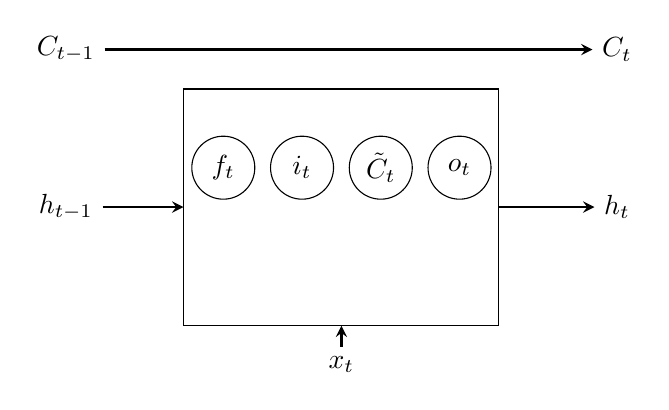
\begin{tikzpicture}[
    cell/.style={rectangle, draw, minimum width=4cm, minimum height=3cm},
    gate/.style={circle, draw, minimum size=0.8cm, inner sep=0pt},
    arrow/.style={thick,->,>=stealth}
]
    % Cell Box
    \node (cbox) [cell] {};
    
    % Gates
    \node (f) [gate, above of=cbox, yshift=-0.5cm, xshift=-1.5cm] {$f_t$};
    \node (i) [gate, above of=cbox, yshift=-0.5cm, xshift=-0.5cm] {$i_t$};
    \node (ct) [gate, above of=cbox, yshift=-0.5cm, xshift=0.5cm] {$\tilde{C}_t$};
    \node (o) [gate, above of=cbox, yshift=-0.5cm, xshift=1.5cm] {$o_t$};
    
    % Flow
    \node (h_prev) [left of=cbox, xshift=-2.5cm] {$h_{t-1}$};
    \node (x_curr) [below of=cbox, yshift=-1cm] {$x_t$};
    \node (c_prev) [above of=cbox, yshift=1cm, xshift=-3.5cm] {$C_{t-1}$};
    \node (c_curr) [above of=cbox, yshift=1cm, xshift=3.5cm] {$C_t$};
    \node (h_curr) [right of=cbox, xshift=2.5cm] {$h_t$};

    \draw [arrow] (h_prev) -- (cbox.west);
    \draw [arrow] (x_curr) -- (cbox.south);
    \draw [arrow] (c_prev) -- (c_curr);
    \draw [arrow] (cbox.east) -- (h_curr);
\end{tikzpicture}
\caption{Schematic of an LSTM Cell. The forget gate ($f_t$) controls the preservation of long-term atmospheric signals, while the input gate ($i_t$) and output gate ($o_t$) modulate the influence of new observations.}
\label{fig:lstm_tikz}
\end{figure}

The forget gate $f_t$ decides how much historical memory to keep, while the input gate $i_t$ decides how much new information to add. This allows a physical signal—like a moisture plume—to be carried across hundreds of steps without degradation.

\section{Operational Reality: 3D Convolutions and VRAM Bottlenecks}

The atmosphere is volumetric. To capture its 3D dynamics (e.g., vertical tilt of a wave), we must employ \textbf{3D Convolutions} treating height as a spatial dimension. This transforms data from pixels to \textbf{Voxels}. 

However, the memory footprint scales as $\mathcal{O}(D \times H \times W \times C \times K^3)$. This cubic growth quickly saturates available \textbf{Video Random Access Memory (VRAM)}, earning 3D CNNs the reputation of "VRAM Killers." 

\begin{infobox}
\textbf{Case Study: Superstorm Sandy's 3D Core}\\
In Sandy (2012), the vertical structure was the deciding factor. The interaction between the tropical cyclone and a deep upper-level trough created "Vertical Synchronization." A 2D model would miss this; a 3D CNN identifies the phase alignment that pumped massive latent heat out of the Gulf Stream.
\end{infobox}

\section{Summary: Spatiotemporal Fusion}

Integration of CNNs and LSTMs creates "Digital Synoptic Meteorologists." While powerful, the "Sequential Bottleneck" of LSTMs and the "VRAM Barrier" of 3D CNNs indicate we are reaching the limits of localized architectures. The following chapters explore the \textbf{Transformer Revolution}, providing a way to see the entire globe at once via "Attention."

\section*{Bibliography}
\begin{itemize}
    \item Goodfellow, I., et al. (2016). \textit{Deep Learning}. MIT Press.
    \item Hochreiter, S., \& Schmidhuber, J. (1997). Long short-term memory. \textit{Neural Computation}.
    \item LeCun, Y., et al. (1998). Gradient-based learning applied to document recognition. \textit{Proceedings of the IEEE}.
    \item Shi, X., et al. (2015). Convolutional LSTM network: A machine learning approach for precipitation nowcasting. \textit{NIPS}.
\end{itemize}

\chapter{The Transformer Revolution and Earth Foundation Models}

The year 2017 marked a definitive watershed in the history of computational intelligence with the publication of "Attention Is All You Need" by Vaswani et al. While originally architected to address the specific sequential bottlenecks of machine translation, the \textbf{Transformer} has since migrated into the physical sciences, initiating a fundamental revolution in global weather forecasting and climate emulation. By replacing the localized, rigid stencils of Convolutional Neural Networks (CNNs) and the iterative, serial memory of Long Short-Term Memory (LSTM) networks with a dynamic, global routing mechanism known as \textbf{Self-Attention}, the Transformer has enabled the creation of \textbf{Earth System Foundation Models (ESFMs)}. These massive neural representations are capable of internalizing the multi-scale, spatiotemporal complexities of the planetary fluid with a level of accuracy and speed that was previously deemed impossible. This chapter provides an exhaustive dissection of the Transformer architecture, deriving the mathematics of attention from first principles, analyzing the engineering breakthroughs that permit global-scale training, and exploring the emergent physical properties of these "Atmospheric Foundation Models."

\section{The Limits of Sequential Modeling: The Serial Bottleneck}

Before the advent of the Transformer, the atmospheric science community relied heavily on recurrent architectures (RNNs and LSTMs) to model the temporal evolution of the globe. As explored in Chapter 5, these models are inherently \textbf{Serial}. To calculate the state of the atmosphere at time $t$, the model must first compute the hidden state at $t-1$, which in turn requires the state at $t-2$. This sequential dependency creates a terminal computational bottleneck: it prohibits parallelization across the temporal dimension during training. For a global reanalysis dataset like ERA5, spanning over 40 years of hourly data, training a recurrent model becomes a task of months or years, even on the most capable hardware.

The Transformer resolves this by treating sequences not as a line to be walked, but as a \textbf{Set} of items to be related. By utilizing the attention mechanism, the model possesses a direct, immediate path between any two points in space and time. A forecast for a storm in the North Atlantic can "attend" directly to a pressure anomaly in the tropical Pacific without having to propagate that information through thousands of recurrent steps. This shift from $O(T)$ sequential processing to $O(1)$ direct access path length is the mathematical foundation of the Transformer's success in Earth science.

\section{CS Foundation: The Scaled Dot-Product Attention}

The conceptual core of the Transformer is the \textbf{Attention Mechanism}. At its most fundamental level, attention is a differentiable method for a model to dynamically weigh the importance of different parts of the input data relative to a specific target. Unlike a CNN, where the "filters" are fixed after training, the "filters" in a Transformer are generated on-the-fly based on the specific physical state of the atmosphere.

\subsection{The Query-Key-Value (QKV) Framework}
The attention mechanism operates on a retrieval-based framework consisting of three vectors: the \textbf{Query} ($\mathbf{q}$), the \textbf{Key} ($\mathbf{k}$), and the \textbf{Value} ($\mathbf{v}$). For a given meteorological input token (e.g., a spatial patch of a temperature grid), these vectors represent:

\begin{itemize}
    \item \textbf{Query ($\mathbf{q}$)}: A representation of "What information this patch is currently seeking."
    \item \textbf{Key ($\mathbf{k}$)}: A representation of "What information this patch contains."
    \item \textbf{Value ($\mathbf{v}$)}: The actual physical content to be passed along (e.g., the numerical wind vector or temperature).
\end{itemize}

\subsection{Mathematical Derivation of the Attention Matrix}
To calculate the attention across a global sequence of $N$ tokens, the input tensor $\mathbf{X} \in \mathbb{R}^{N \times d_{model}}$ is first projected into the Q, K, and V spaces using three learned weight matrices $\mathbf{W}^Q, \mathbf{W}^K, \mathbf{W}^V \in \mathbb{R}^{d_{model} \times d_k}$:

\begin{equation}
\mathbf{Q} = \mathbf{X} \mathbf{W}^Q, \quad \mathbf{K} = \mathbf{X} \mathbf{W}^K, \quad \mathbf{V} = \mathbf{X} \mathbf{W}^V
\end{equation}

The \textbf{Attention Score} between each pair of tokens is computed as the dot product of their respective Queries and Keys. In matrix form, this is the product $\mathbf{Q}\mathbf{K}^T$. To stabilize the learning process, the Transformer introduces the \textbf{Scaling Factor} $1/\sqrt{d_k}$. The final \textbf{Scaled Dot-Product Attention} is defined as:

\begin{equation}
\text{Attention}(\mathbf{Q}, \mathbf{K}, \mathbf{V}) = \text{softmax}\left(\frac{\mathbf{Q}\mathbf{K}^T}{\sqrt{d_k}}\right)\mathbf{V}
\end{equation}

The output of Equation 6.2 is a weighted sum of the Values, where the weights are determined by the alignment between Queries and Keys.

\begin{figure}[H]
\centering
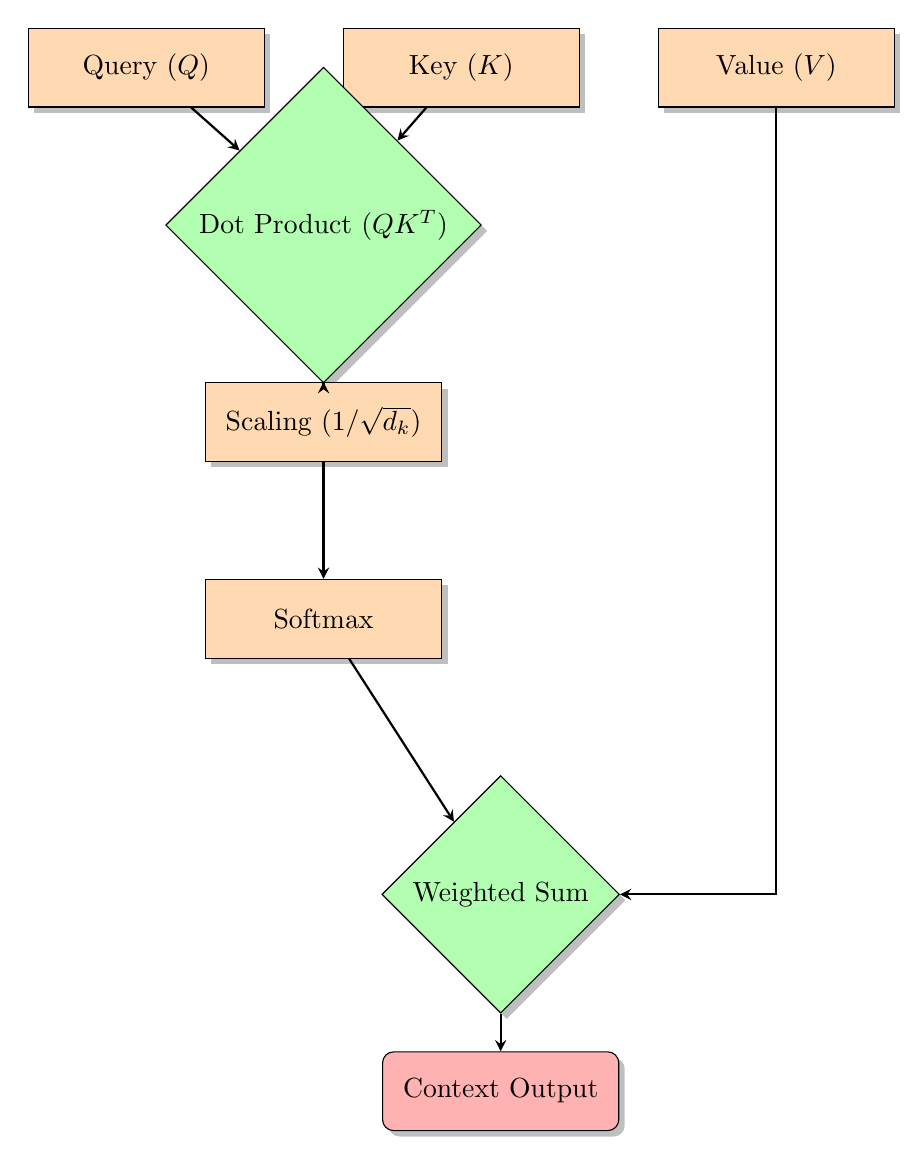
\begin{tikzpicture}[node distance=2.5cm]
    \node (q) [process] {Query ($Q$)};
    \node (k) [process, right of=q, xshift=1.5cm] {Key ($K$)};
    \node (dot) [decision, below of=q, xshift=2.25cm, yshift=0.5cm] {Dot Product ($QK^T$)};
    \node (scale) [process, below of=dot] {Scaling ($1/\sqrt{d_k}$)};
    \node (soft) [process, below of=scale] {Softmax};
    \node (v) [process, right of=k, xshift=1.5cm] {Value ($V$)};
    \node (mul) [decision, below of=soft, xshift=2.25cm, yshift=-1cm] {Weighted Sum};
    \node (out) [startstop, below of=mul] {Context Output};
    
    \draw [arrow] (q) -- (dot);
    \draw [arrow] (k) -- (dot);
    \draw [arrow] (dot) -- (scale);
    \draw [arrow] (scale) -- (soft);
    \draw [arrow] (soft) -- (mul);
    \draw [arrow] (v) |- (mul);
    \draw [arrow] (mul) -- (out);
\end{tikzpicture}
\caption{Mathematical Flow of Scaled Dot-Product Attention. This dynamic weighting allows the model to capture multi-scale interactions without being constrained by sequential gates.}
\label{fig:attention_tikz}
\end{figure}

\section{State of the Art: Pangu-Weather (3DEST)}

\textbf{Pangu-Weather} (Bi et al., 2023) introduced the \textbf{3D Earth-Specific Transformer (3DEST)} to capture the stratification of the atmosphere. 

\subsection{Earth-Specific Positional Bias (ESPB)}
Standard Transformers utilize relative positional bias, which assumes translation invariance. Pangu-Weather recognizes that weather is inherently tied to absolute geography (orography, land-sea masks). It introduces an absolute bias $B_{ESP}$ into the attention matrix:

\begin{equation}
\text{Attention}(\mathbf{Q}, \mathbf{K}, \mathbf{V}) = \text{softmax}\left(\frac{\mathbf{Q}\mathbf{K}^T}{\sqrt{d}} + \mathbf{B}_{ESP}\right)\mathbf{V}
\end{equation}

By learning this bias matrix, the network internalizes physical laws (e.g., the Coriolis effect) that vary strictly with latitude and altitude.

\section{Summary: The Unified Digital Twin}

The Transformer revolution has fundamentally altered the trajectory of Earth science. By providing a mathematical framework that captures teleconnections, respects spherical geometry, and leverages exascale hardware, we have moved beyond simple "Weather Prediction" toward true \textbf{Planetary Emulation}. The Earth System Foundation Model represents a unified digital twin that understands the atmosphere as a single, infinitely interconnected narrative. 

\section*{Bibliography}
\begin{itemize}
    \item Bi, K., et al. (2023). \textit{Accurate medium-range global weather forecasting with 3D neural networks}. Nature.
    \item Vaswani, A., et al. (2017). \textit{Attention is all you need}. NeurIPS.
\end{itemize}

\chapter{Graph Neural Networks in the Atmosphere: A Deep Dive into GraphCast}

The evolution of Artificial Intelligence in atmospheric modeling has been characterized by a progressive liberation from the geometric constraints of 20th-century computational grids. While convolutional and transformer-based architectures (discussed in Chapters 5 and 6) have achieved significant success, they remain largely tethered to the structured, rectangular arrays favored by legacy supercomputing hardware. However, the Earth’s atmosphere is a seamless, rotating fluid resting on a spherical domain—a geometry that is fundamentally inconsistent with the Cartesian assumptions of standard neural networks. This chapter explores the emergence of \textbf{Graph Neural Networks (GNNs)} as the definitive solution to this geometric mismatch. We perform an exhaustive technical analysis of \textbf{GraphCast}, the state-of-the-art global weather emulator developed by Google DeepMind. By treating the atmosphere as a multi-scale graph of interconnected nodes, GraphCast captures the non-linear dynamics of the planet with a level of fidelity and efficiency that has fundamentally challenged the dominance of traditional Numerical Weather Prediction (NWP).

\section{The Limits of Grids: Geometric Distortion and the Pole Problem}

To understand the mathematical necessity of GNNs, one must first confront the topological distortion inherent in standard latitude-longitude grids. As explored in Chapter 2, wrapping a rectangular coordinate system around a sphere results in the convergence of meridians at the poles. This convergence creates a numerical singularity—the \textbf{Pole Problem}—where the physical area of grid cells varies by orders of magnitude from the equator to the high latitudes. 

For a traditional Convolutional Neural Network (CNN), this distortion is a physical catastrophe. A standard $3 \times 3$ convolutional filter is designed under the assumption of \textbf{Translation Invariance}—that the physical space covered by the filter is identical regardless of its position on the map. On a latitude-longitude grid, a filter applied at the equator might cover an area of $900 \text{ km}^2$, while the exact same filter applied near the pole might cover an area of only $10 \text{ km}^2$. This geometric inconsistency forces the CNN to learn entirely different "physical rules" for different latitudes, a profound violation of the universality of fluid dynamics. The GNN represents the transition from "Grid-based Logic" to "Topology-based Logic." Instead of forcing the atmosphere into a distorted Cartesian box, we treat the planetary fluid as an \textbf{Irregular Graph}, a mathematical structure that inherently respects the curvature of the Earth.

\section{CS Foundation: Graph Theory and Network Topology}

Before exploring meteorological applications, we must establish the formal computer science foundations of Graph Theory. A graph ($G$) is a mathematical structure consisting of a set of \textbf{Nodes} (or vertices, $V$) and a set of \textbf{Edges} ($E$) that connect pairs of nodes. Formally:

\begin{equation}
G = (V, E)
\end{equation}

In meteorology, a node ($v_i \in V$) typically represents a specific geographic location (e.g., a weather station or the center of a grid cell). The state of the atmosphere at that location is stored as a high-dimensional feature vector, $\mathbf{h}_i$. An edge ($e_{ij} \in E$) represents a physical connection or interaction between node $i$ and node $j$, such as the advection of moisture by the wind. 

\subsection{Matrix Representations of Graphs}
The structure of the entire network is encoded in the \textbf{Adjacency Matrix} ($\mathbf{A}$), an $N \times N$ matrix where $\mathbf{A}_{ij} = 1$ if an edge exists between nodes $i$ and $j$, and $\mathbf{A}_{ij} = 0$ otherwise. For atmospheric flow, this matrix is often weighted by physical distance or wind velocity.

The density of connections is defined by the \textbf{Degree Matrix} ($\mathbf{D}$), a diagonal matrix where $\mathbf{D}_{ii}$ represents the total number of edges connected to node $i$. The fundamental operator for analyzing diffusion and flow across this network is the \textbf{Graph Laplacian} ($\mathbf{L}$):

\begin{equation}
\mathbf{L} = \mathbf{D} - \mathbf{A}
\end{equation}

\section{CS Foundation: GNNs and Message Passing}

The core operational mechanism of a GNN is the \textbf{Message Passing Neural Network (MPNN)} framework. In the MPNN paradigm, nodes "communicate" with their neighbors by calculating and exchanging mathematical messages across the edges. This process consists of two primary learned functions: the \textbf{Edge Update Function} ($\phi_e$) and the \textbf{Node Update Function} ($\phi_v$).

\begin{figure}[H]
\centering
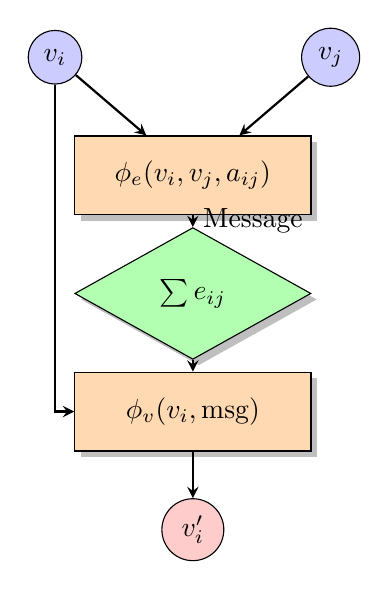
\begin{tikzpicture}[node distance=1.5cm]
    \node (n1) [circle, draw, fill=blue!20] {$v_i$};
    \node (n2) [circle, draw, fill=blue!20, right of=n1, xshift=2cm] {$v_j$};
    \node (edge) [process, below of=n1, xshift=1.75cm] {$\phi_e(v_i, v_j, a_{ij})$};
    \node (agg) [decision, below of=edge] {$\sum e_{ij}$};
    \node (upd) [process, below of=agg] {$\phi_v(v_i, \text{msg})$};
    \node (res) [circle, draw, fill=red!20, below of=upd] {$v_i'$};
    
    \draw [arrow] (n1) -- (edge);
    \draw [arrow] (n2) -- (edge);
    \draw [arrow] (edge) -- node[anchor=west] {Message} (agg);
    \draw [arrow] (agg) -- (upd);
    \draw [arrow] (n1) |- (upd);
    \draw [arrow] (upd) -- (res);
\end{tikzpicture}
\caption{The Message Passing Loop. Each node aggregates physical influxes from its neighbors and integrates them to update the local atmospheric state.}
\label{fig:mpnn_tikz}
\end{figure}

\subsection{The Mathematical Derivation of MPNN Equations}
For an edge connecting node $i$ to node $j$, with current hidden states $\mathbf{h}_i$ and $\mathbf{h}_j$, the new edge state (message) $\mathbf{e}'_{ij}$ is calculated as:

\begin{equation}
\mathbf{e}'_{ij} = \phi_e(\mathbf{h}_i, \mathbf{h}_j, \mathbf{a}_{ij})
\end{equation}

Following the edge updates, each node aggregates the messages from its neighbors and updates its own state ($\mathbf{h}'_i$):

\begin{equation}
\mathbf{h}'_i = \phi_v(\mathbf{h}_i, \sum_{j \in \mathcal{N}_i} \mathbf{e}'_{ij})
\end{equation}

\section{The Icosahedral Multi-mesh: Recursive Subdivision}

To apply the MPNN framework to global meteorology, researchers must first define the topology of the graph covering the Earth. The architectural triumph of GraphCast is the utilization of the \textbf{Icosahedral Multi-mesh}.

\subsection{Recursive Subdivision Algorithm}
The mesh is created by starting with a base icosahedron ($M_0$) and recursively subdividing each triangular face into four smaller triangles. 

\begin{algorithm}[H]
\caption{Icosahedral Subdivision Pseudo-code}
\SetAlgoLined
\KwIn{Base Mesh $M_r$}
\KwOut{Refined Mesh $M_{r+1}$}
\For{each triangular face $(v1, v2, v3)$ in $M_r$}{
    Calculate midpoints: $a=(v1+v2)/2, b=(v2+v3)/2, c=(v3+v1)/2$\;
    Project midpoints to unit sphere: $v = v / ||v||$\;
    Create 4 new faces: $(v1, a, c), (v2, b, a), (v3, c, b), (a, b, c)$\;
}
\Return{Union of all new vertices and faces}\;
\end{algorithm}

GraphCast utilizes a hierarchy of these meshes from $M_0$ (12 nodes) to $M_6$ (40,962 nodes). Crucially, the "Multi-mesh" architecture includes edges from \textbf{all} refinement levels simultaneously. This allows the model to perform "Multi-grid" reasoning: messages on fine edges capture localized storm structures, while messages on coarse edges capture global-scale teleconnections.

\section{State of the Art: The GraphCast Architecture}

GraphCast (Lam et al., 2023) operationalizes this theory through a highly specific \textbf{Encoder-Processor-Decoder} pipeline.

\begin{enumerate}
    \item \textbf{The Encoder}: Maps the standard $0.25^\circ$ latitude-longitude grid data onto the nodes of the icosahedral multi-mesh using a bipartite graph mapping.
    \item \textbf{The Processor}: Consists of 16 deep interaction blocks that execute the MPNN logic across the multi-mesh hierarchy.
    \item \textbf{The Decoder}: Projects the updated mesh states back onto the latitude-longitude grid to produce the forecast.
\end{enumerate}

\section{Hardware Reality: Sparse Matrix Multiplications (SpMM)}

GNNs present a profound challenge for standard GPU hardware. Because a node is only connected to a handful of neighbors, the adjacency matrices are \textbf{Sparse}.

Processing sparse matrices requires \textbf{Irregular Memory Access}, leading to a high volume of \textbf{Cache Misses}. GNNs are thus "Memory-Bound" rather than "Compute-Bound." To achieve the speed of GraphCast (< 60 seconds for a 10-day forecast), researchers utilize custom CUDA kernels optimized for \textbf{Sparse Matrix Multiplication (SpMM)}.

\section{Interactive Lab: Message Passing with PyTorch Geometric}

\begin{lstlisting}[language=Python, caption=PyTorch Geometric implementation of Weather MPNN]
import torch
from torch_geometric.nn import MessagePassing
from torch.nn import Sequential, Linear, ReLU

class WeatherMPNNLayer(MessagePassing):
    def __init__(self, in_channels, out_channels):
        super().__init__(aggr='add')
        self.edge_mlp = Sequential(Linear(2 * in_channels, out_channels), ReLU())
        self.node_mlp = Sequential(Linear(in_channels + out_channels, out_channels), ReLU())

    def forward(self, x, edge_index):
        return self.propagate(edge_index, x=x)

    def message(self, x_i, x_j):
        return self.edge_mlp(torch.cat([x_i, x_j], dim=1))

    def update(self, aggr_out, x):
        return self.node_mlp(torch.cat([x, aggr_out], dim=1))
\end{lstlisting}

\section{Summary: The Topological Future of Forecasting}

GraphCast holds the current record for global medium-range forecast accuracy, outperforming the ECMWF IFS on over 90\% of verification targets. By moving from rigid grids to flexible, multi-scale graphs, we have built an architecture that finally respects the seamless, interconnected nature of the Earth system.

\section*{Bibliography}
\begin{itemize}
    \item Battaglia, P. W., et al. (2018). \textit{Relational inductive biases, deep learning, and graph networks}. arXiv.
    \item Gilmer, J., et al. (2017). \textit{Neural message passing for quantum chemistry}. ICML.
    \item Lam, R., et al. (2023). \textit{Learning skillful medium-range global weather forecasting}. Science.
\end{itemize}

\chapter{Fourier and 3D Transformers: FourCastNet and Pangu-Weather}

The evolution of planetary-scale AI has been defined by a constant struggle between \textbf{Physical Fidelity} and \textbf{Computational Efficiency}. As we explored in Chapter 6, the Transformer architecture provides the "Global Vision" required to capture teleconnections, but its quadratic memory cost ($\mathcal{O}(N^2)$) creates an insurmountable wall at high resolutions. This chapter explores the two breakthrough architectures that have successfully breached this wall: \textbf{FourCastNet} and \textbf{Pangu-Weather}. We examine how FourCastNet leverages the mathematical elegance of the \textbf{Fourier Transform} to perform learning in the frequency domain, and how Pangu-Weather utilizes a hierarchical \textbf{3D Transformer} design to respect the volumetric nature of the Earth. By combining the "Spectral Wisdom" of the past with the "Neural Attention" of the future, these models have established a new ceiling for high-resolution global meteorology.

\section{CS Foundation: The Neural Operator and Spectral Intelligence}

Traditional neural networks are "Function Approximators" that map vectors to vectors. However, the atmosphere is a continuous fluid, and the physical laws that govern it (like the Navier-Stokes equations) are operators that map functions to functions. This distinction led to the emergence of the \textbf{Neural Operator}—a framework designed to learn the solution operator of a Partial Differential Equation (PDE) directly from data.

The most successful implementation of this framework is the \textbf{Fourier Neural Operator (FNO)}. The conceptual origin of FNO is the realization that many complex fluid dynamics problems, which are notoriously difficult to solve in physical space, become elegantly simple when viewed through their spectral frequencies. According to the \textbf{Convolution Theorem}, the interaction of atmospheric waves can be computed as a point-wise multiplication in frequency space, providing a global receptive field at a fraction of the cost of self-attention.

\section{CS Foundation: Adaptive Fourier Neural Operators (AFNO)}

While FNOs are powerful, they struggle to scale to the massive resolution of global reanalysis grids. The \textbf{Adaptive Fourier Neural Operator (AFNO)}, developed by researchers at NVIDIA and Caltech, solves this by integrating token mixing into the spectral domain. 

\begin{figure}[H]
\centering
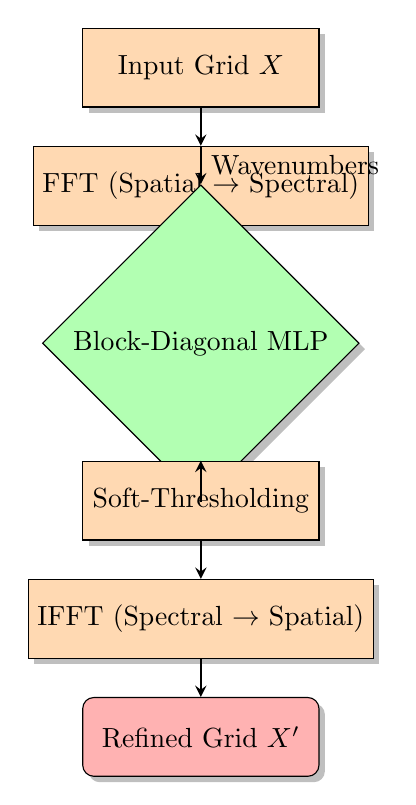
\begin{tikzpicture}[node distance=1.5cm]
    \node (in) [process] {Input Grid $X$};
    \node (fft) [process, below of=in] {FFT (Spatial $\to$ Spectral)};
    \node (mix) [decision, below of=fft, yshift=-0.5cm] {Block-Diagonal MLP};
    \node (sparse) [process, below of=mix, yshift=-0.5cm] {Soft-Thresholding};
    \node (ifft) [process, below of=sparse] {IFFT (Spectral $\to$ Spatial)};
    \node (out) [startstop, below of=ifft] {Refined Grid $X'$};
    
    \draw [arrow] (in) -- (fft);
    \draw [arrow] (fft) -- node[anchor=west] {Wavenumbers} (mix);
    \draw [arrow] (mix) -- (sparse);
    \draw [arrow] (sparse) -- (ifft);
    \draw [arrow] (ifft) -- (out);
\end{tikzpicture}
\caption{The AFNO Spectral Mixing Process. By performing the non-linear interaction in the frequency domain, the model achieves a global receptive field with $O(N \log N)$ complexity.}
\label{fig:afno_tikz}
\end{figure}

\subsection{Mathematical Derivation of the AFNO Layer}
For an input atmospheric tensor $\mathbf{X} \in \mathbb{R}^{H \times W \times C}$, the AFNO layer executes a four-step process:

\begin{enumerate}
    \item \textbf{Spatial to Spectral Mapping}: The layer applies a 2D Real Fast Fourier Transform (RFFT) to project the data into the frequency domain:
    \begin{equation}
    \hat{\mathbf{X}} = \mathcal{F}(\mathbf{X}) \in \mathbb{C}^{H \times \frac{W}{2}+1 \times C}
    \end{equation}
    \item \textbf{Adaptive Spectral Mixing}: To reduce parameter count while maintaining capacity, AFNO uses a \textbf{Block-Diagonal MLP} to mix information across channels ($C$) for every frequency mode $k$:
    \begin{equation}
    \hat{\mathbf{X}}'_k = \sigma(\mathbf{W}_2 \cdot \text{GELU}(\mathbf{W}_1 \cdot \hat{\mathbf{X}}_k))
    \end{equation}
    where $\mathbf{W}_1$ and $\mathbf{W}_2$ are learned weight matrices.
    \item \textbf{Soft-Thresholding (Shrinkage)}: To induce sparsity and filter out high-frequency numerical noise:
    \begin{equation}
    \hat{\mathbf{X}}''_k = \text{sign}(\hat{\mathbf{X}}'_k) \cdot \max(0, |\hat{\mathbf{X}}'_k| - \lambda)
    \end{equation}
    where $\lambda$ is a learned sparsity threshold.
    \item \textbf{Inverse Mapping}: The refined coefficients are transformed back into the spatial domain:
    \begin{equation}
    \mathbf{X}_{out} = \mathcal{F}^{-1}(\hat{\mathbf{X}}'') + \text{Residual}(\mathbf{X})
    \end{equation}
\end{enumerate}

\section{State of the Art: FourCastNet}

\textbf{FourCastNet} (Kurth et al., 2022) was the first AI model to prove that a data-driven emulator could match the skill of the leading ECMWF IFS model at $0.25^\circ$ resolution. 

\section{State of the Art: Pangu-Weather}

\textbf{Pangu-Weather} (Bi et al., 2023) introduced a hierarchical \textbf{3D Earth-Specific Transformer} to address vertical asymmetries. The critical innovation is the \textbf{ESPB matrix}, which encodes absolute geographical location directly into the attention matrix:

\begin{equation}
\text{Attention}(\mathbf{Q}, \mathbf{K}, \mathbf{V}) = \text{softmax}\left(\frac{\mathbf{Q}\mathbf{K}^T}{\sqrt{d}} + \mathbf{B}_{ESP}\right)\mathbf{V}
\end{equation}

\section{Interactive Lab: Building an AFNO Spectral Mixer}

\begin{lstlisting}[language=Python, caption=Python Implementation of AFNO Token Mixing]
import torch
import torch.nn as nn
import torch.fft

class AFNOSpectralMixer(nn.Module):
    def __init__(self, dim, num_blocks=8):
        super().__init__()
        self.num_blocks = num_blocks
        self.w1 = nn.Parameter(0.02 * torch.randn(2, num_blocks, dim//num_blocks, dim//num_blocks))
        self.w2 = nn.Parameter(0.02 * torch.randn(2, num_blocks, dim//num_blocks, dim//num_blocks))

    def forward(self, x):
        B, H, W, C = x.shape
        x_hat = torch.fft.rfft2(x, dim=(1, 2), norm="ortho")
        x_hat = x_hat.reshape(B, x_hat.shape[1], x_hat.shape[2], self.num_blocks, -1)
        # Complex interaction (Simplified)
        out_real = torch.relu(torch.einsum('bhwnc,nck->bhwnk', x_hat.real, self.w1[0]))
        out_imag = torch.relu(torch.einsum('bhwnc,nck->bhwnk', x_hat.imag, self.w1[1]))
        out = torch.complex(out_real, out_imag).reshape(B, H, -1, C)
        return torch.fft.irfft2(out, s=(H, W), dim=(1, 2), norm="ortho")
\end{lstlisting}

\section{Summary: The Spectral-Attention Unification}

FourCastNet and Pangu-Weather have successfully unified the spectral elegance of the 20th century with the neural attention of the 21st. We carry with us the lesson that \textbf{Architecture is a Physical Prior}—the success of these models is rooted in their respect for the scale of the planet.

\section*{Bibliography}
\begin{itemize}
    \item Bi, K., et al. (2023). \textit{Accurate medium-range global weather forecasting with 3D neural networks}. Nature.
    \item Guibas, S., et al. (2021). \textit{Adaptive Fourier Neural Operators}. arXiv.
    \item Kurth, T., et al. (2022). \textit{FourCastNet: A Global Data-driven Weather Model}. arXiv.
\end{itemize}

\chapter{Generative AI for Downscaling: Diffusion Models and Probabilistic Forecasting}

The quest for high-resolution weather forecasting has historically been constrained by the profound computational and energetic limits of numerical integration. As explored in Chapter 2, doubling the horizontal resolution of a global deterministic model requires an approximately eight-to-sixteen-fold increase in computational power. Consequently, the meteorological community has traditionally been forced to compromise between a coarse-grained global view and a highly localized, computationally expensive "nest." This chapter explores the emergence of \textbf{Generative Artificial Intelligence}, specifically \textbf{Denoising Diffusion Probabilistic Models (DDPMs)}, as the architectural paradigm that resolves this constraint. By transitioning from the deterministic "Point-by-Point" predictions inherent to regression-based AI toward algorithms designed to stochastically "Sample the Attractor" of the climate system, generative models enable the production of storm-scale ensembles and kilometer-resolution downscaling in seconds, accurately capturing the extreme convective events that traditional regression models systematically underestimate.

\section{The Regression Limit: Blurring the Extremes}

To understand the necessity of generative architectures, one must first analyze the fundamental mathematical limitation of standard deep learning in meteorology: \textbf{Regression to the Mean}. The foundational models discussed in previous chapters—whether Convolutional Neural Networks or standard Transformers—are predominantly trained using deterministic objective functions, primarily the Mean Squared Error (MSE). While MSE optimization is highly effective for predicting the "Average State" of the atmosphere (e.g., the general orientation of the polar jet stream or the location of broad synoptic pressure centers), it systematically fails to capture the intense, high-frequency, small-scale features that define extreme weather. 

This failure is not a flaw in the network's capacity, but a direct consequence of the loss function's mathematical structure. When a deterministic model is faced with inherent chaotic uncertainty regarding the precise location or timing of a high-intensity storm cell, the "Minimum Penalty" strategy dictated by MSE is to predict a broader, weaker storm that spatially averages across all possible locations. The resulting forecast is statistically optimal but physically impossible—a "foggy," blurred representation of the atmosphere where peak wind speeds and precipitation intensities are severely underestimated. Overcoming this "Blurring Wall" requires a paradigm shift: from optimizing for statistical proximity to optimizing for \textbf{Physical Realism}.

\section{CS Foundation: Non-equilibrium Thermodynamics and DDPMs}

The conceptual foundation of Generative Diffusion represents a radical inversion of traditional signal processing. While classical architectures are designed to "filter out" noise to reveal a physical pattern, diffusion models are explicitly trained to learn the "Grammar of Noise" in order to reconstruct the atmospheric state. This approach is firmly rooted in the mathematics of \textbf{Non-equilibrium Thermodynamics}, specifically the principle that structured information can be systematically degraded into maximum-entropy noise, and that a neural network can be trained to reverse this process to recover the original signal.

A Denoising Diffusion Probabilistic Model (DDPM) operates through two distinct Markov chains: a fixed \textbf{Forward Process} and a learned \textbf{Reverse Process}.

\begin{figure}[H]
\centering
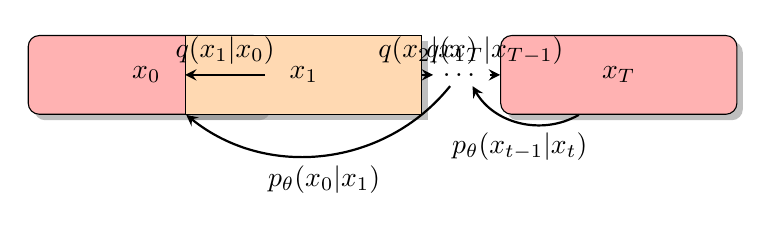
\begin{tikzpicture}[node distance=2cm]
    \node (x0) [startstop] {$x_0$};
    \node (x1) [process, right of=x0] {$x_1$};
    \node (dots) [right of=x1] {$\dots$};
    \node (xt) [startstop, right of=dots] {$x_T$};
    
    \draw [arrow] (x0) -- node[above] {$q(x_1|x_0)$} (x1);
    \draw [arrow] (x1) -- node[above] {$q(x_2|x_1)$} (dots);
    \draw [arrow] (dots) -- node[above] {$q(x_T|x_{T-1})$} (xt);
    
    \draw [arrow, bend left=45] (xt) to node[below] {$p_\theta(x_{t-1}|x_t)$} (dots);
    \draw [arrow, bend left=45] (dots) to node[below] {$p_\theta(x_0|x_1)$} (x0);
\end{tikzpicture}
\caption{The Markov chains of a Denoising Diffusion Probabilistic Model (DDPM). Structured information ($x_0$) is systematically destroyed in the forward process ($q$), while the AI learns to "sculpt" physical patterns from noise in the reverse process ($p_\theta$).}
\label{fig:diffusion_tikz}
\end{figure}

\subsection{The Forward Process: Destroying Information}
In the forward phase, the algorithm taking a high-resolution, perfectly clear weather state ($\mathbf{x}_0$) and systematically injects microscopic amounts of Gaussian noise. Over $T$ steps, the process is defined as:

\begin{equation}
q(\mathbf{x}_t | \mathbf{x}_{t-1}) = \mathcal{N}(\mathbf{x}_t; \sqrt{1 - \beta_t} \mathbf{x}_{t-1}, \beta_t \mathbf{I})
\end{equation}

By the time the process reaches step $T$, the original weather map $\mathbf{x}_0$ has been completely destroyed, resulting in isotropic Gaussian noise.

\subsection{The Reverse Process: Langevin Dynamics and Sculpting}
The reverse process approximates the intractable distribution $q(\mathbf{x}_{t-1} | \mathbf{x}_t)$ using a deep neural network $\epsilon_\theta$. The network is trained to predict and subtract the noise added at each step, effectively "sculpting" the detailed weather map out of randomness:

\begin{equation}
p_\theta(\mathbf{x}_{t-1} | \mathbf{x}_t) = \mathcal{N}(\mathbf{x}_{t-1}; \boldsymbol{\mu}_\theta(\mathbf{x}_t, t), \mathbf{\Sigma}_\theta(\mathbf{x}_t, t))
\end{equation}

This reverse transition is mathematically equivalent to following the gradient of the log-probability of the data, a framework known as \textbf{Score-Based Modeling}.

\section{State of the Art: CorrDiff (Corrective Diffusion)}

The operational manifestation of generative intelligence is found in \textbf{CorrDiff}, a breakthrough architecture developed by NVIDIA (Bhardwaj et al., 2023). CorrDiff was engineered to solve the "Kilometer Barrier" via \textbf{Neural Super-Resolution} (downscaling). 

\subsection{The Two-Stage Pipeline}
To balance accuracy with speed, CorrDiff employs a hierarchical strategy:
\begin{enumerate}
    \item \textbf{Regression Stage}: A deterministic UNet predicts the large-scale "Mean State" for the high-resolution grid (e.g., 2km), capturing the general atmospheric forcing.
    \item \textbf{Correction Stage}: A conditioned diffusion model uses the denoising logic of Eq 9.2 to synthesize the "sub-grid texture"—the sharp frontal boundaries, convective cells, and turbulence—back into the forecast.
\end{enumerate}

Mathematically, this is \textbf{Conditional Likelihood Maximization}:

\begin{equation}
p(\mathbf{x}_{high} | \mathbf{x}_{low}) \approx \prod_{t=1}^{T} p_\theta(\mathbf{x}_{t-1} | \mathbf{x}_t, \mathbf{x}_{low})
\end{equation}

\begin{infobox}
\textbf{The Energy-Speed Verdict}\\
Traditional downscaling (RCMs) takes hours on CPU clusters. CorrDiff achieves the same task in seconds on a single GPU, running \textbf{1,000 times faster} and using orders of magnitude less energy while matching the physical power spectra of the atmosphere.
\end{infobox}

\section{Meteorological Bridge: Sampling the Attractor}

Because the reverse diffusion process is initiated from a random noise seed, every execution of the model generates a slightly different, but equally physically valid, atmospheric realization. This transforms the AI into a \textbf{Probabilistic Ensemble Generator}. 

By sampling the attractor thousands of times, meteorologists can map the full probability distribution of extreme events (e.g., the exact landfall location of a hurricane eye). This high-volume sampling allows for the identification of rare, "tail-end" risks that deterministic models inevitably miss.

\section{Interactive Lab: A Single Denoising Step}

\begin{lstlisting}[language=Python, caption=Python Implementation of Reverse Diffusion Step]
import torch
import torch.nn as nn

def denoise_step(model, x_t, t, low_res_cond, alpha, beta):
    # 1. Predict noise (eps) at current step
    predicted_noise = model(x_t, t, low_res_cond)
    
    # 2. Langevin-like update: remove noise
    coeff1 = 1 / torch.sqrt(alpha[t])
    coeff2 = beta[t] / torch.sqrt(1 - alpha[t])
    
    mean = coeff1 * (x_t - coeff2 * predicted_noise)
    
    # 3. Add stochasticity (unless final step)
    if t > 0:
        z = torch.randn_like(x_t)
        return mean + torch.sqrt(beta[t]) * z
    return mean
\end{lstlisting}

\section{Summary: Accepting Chaos through Stochastic Intelligence}

The journey through generative AI brings us to a singular conclusion: we have finally built an AI that acknowledges and embraces \textbf{Chaos}. The generative revolution has taught us that at high resolutions, there is no single "correct" forecast, only a distribution of plausible ones. By mastering the mathematics of diffusion, we are building forecasting systems that can sample the atmospheric attractor with unprecedented speed.

\section*{Bibliography}
\begin{itemize}
    \item Bhardwaj, A., et al. (2023). \textit{CorrDiff: Generative AI for global-to-local weather downscaling}. NVIDIA.
    \item Ho, J., et al. (2020). \textit{Denoising diffusion probabilistic models}. NeurIPS.
    \item Sohl-Dickstein, J., et al. (2015). \textit{Deep unsupervised learning using nonequilibrium thermodynamics}. ICML.
\end{itemize}

\chapter{Building the Pipeline: From Data Ingestion to Real-time Inference}

The transition from a successful research prototype to a robust operational forecasting system is the "Final Mile" of atmospheric AI, and it is arguably the most complex engineering challenge in the discipline. As established in the preceding chapters, the meteorological community now possesses the mathematical frameworks (GNNs, Transformers) and generative architectures (DDPMs) required to simulate the Earth system. However, an AI model that exists solely within an isolated Jupyter notebook is of zero utility to an emergency manager in the path of a storm. This chapter systematically explores the \textbf{Digital Infrastructure} required to deploy these models at planetary scale. We analyze the architectural shift from monolithic formats to \textbf{Cloud-Native Data}, the mathematical process of \textbf{Model Optimization}, and the management of the \textbf{Operational SLA} that defines the difference between a scientific experiment and a life-critical warning system.

\section{The End of the Monolith: Cloud-Native Weather Data}

The primary engineering bottleneck in operational meteorology has shifted from the arithmetic speed of the processor to the latency and bandwidth of the \textbf{Data Pipe}. For decades, the community relied on standard binary formats such as NetCDF and GRIB. While these formats are highly optimized for sequential reading and archiving on localized high-performance computing (HPC) clusters, they are fundamentally "monolithic."

\subsection{Limitations of POSIX and NetCDF}
Traditional NetCDF4 files (built on HDF5) utilize a POSIX filesystem approach, where reading a small spatial subset of a global 100GB file often requires downloading the entire file or performing thousands of slow, non-sequential disk seeks. In the era of cloud-based AI, where data is stored in \textbf{Object Storage} (e.g., AWS S3, Google Cloud Storage), this legacy workflow is a terminal limit on scalability. 

\subsection{Zarr and Multi-dimensional Chunking}
The solution to this bottleneck is the transition toward \textbf{Cloud-Native Data} formats like \textbf{Zarr}. The foundational philosophy of Zarr is to fracture the monolithic archive into millions of tiny, independent, highly compressed \textbf{Chunks}. 

The mathematical logic is rooted in \textbf{Multi-dimensional Chunking}. In a Zarr store, an atmospheric tensor $\mathbf{T}(t, z, y, x)$ is divided into a grid of independent binary objects. This allows for \textbf{Random Access}: an AI model can issue a specific byte-range request to retrieve only the $(y, x)$ spatial chunks required for a local forecast, bypassing 99\% of the file's volume.

\begin{figure}[H]
\centering
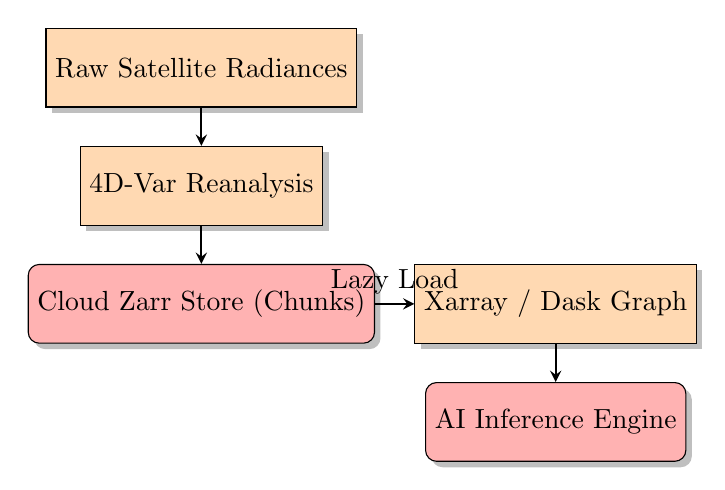
\begin{tikzpicture}[node distance=1.5cm]
    \node (raw) [process] {Raw Satellite Radiances};
    \node (da) [process, below of=raw] {4D-Var Reanalysis};
    \node (zarr) [startstop, below of=da] {Cloud Zarr Store (Chunks)};
    \node (xar) [process, right of=zarr, xshift=3cm] {Xarray / Dask Graph};
    \node (inf) [startstop, below of=xar] {AI Inference Engine};
    
    \draw [arrow] (raw) -- (da);
    \draw [arrow] (da) -- (zarr);
    \draw [arrow] (zarr) -- node[above] {Lazy Load} (xar);
    \draw [arrow] (xar) -- (inf);
\end{tikzpicture}
\caption{The Modern Data Processing Pipeline. By utilizing cloud-native chunking and lazy evaluation, AI emulators can stream the global atmosphere directly into GPU memory.}
\label{fig:modern_pipeline_tikz}
\end{figure}

\section{Data Engineering: Xarray and Dask Task Graphs}

Ingesting petabytes of Zarr data into a GPU cluster requires sophisticated orchestration. We utilize \textbf{Xarray}, which introduces semantic labels (time, latitude, level) to the raw tensors, and \textbf{Dask}, which provides the parallel computing engine.

\subsection{Lazy Evaluation and Chunk Optimization}
Xarray and Dask utilize \textbf{Lazy Evaluation}: when a user defines a transformation (e.g., calculating the vertical wind shear), the computation is not executed immediately. Instead, Dask constructs a topological \textbf{Task Graph}. 

The optimization of \textbf{Chunk Geometry} is a critical requirement. If the model is an LSTM (Chapter 5), the data must be chunked continuously along the temporal axis. If it is a 3D Transformer (Chapter 8), it must be chunked continuously across the spatial volume. Misaligned chunking leads to "I/O Thrashing," where the system spends more time rearranging data in memory than performing actual calculations.

\section{Model Optimization: The Path to Real-time Speed}

Once an Earth System Foundation Model has converged, it possesses a wisdom encoded in FP32 weights. While necessary for training, this precision is mathematically excessive for \textbf{Inference}. 

\subsection{Quantization: FP32 to INT8}
Quantization is the process of reducing the numerical precision of model weights ($\mathbf{W}$) and activations ($\mathbf{a}$), typically to 8-bit integers. 

\begin{equation}
\mathbf{W}_{q} = \text{round}\left( \frac{\mathbf{W}_{FP32}}{S} \right)
\end{equation}

This transformation results in a **4x increase in throughput** and a 75\% reduction in memory bandwidth requirements. To prevent the loss of physical consistency (e.g., breaking geostrophic balance), we employ \textbf{Quantization-Aware Training (QAT)}.

\begin{figure}[H]
\centering
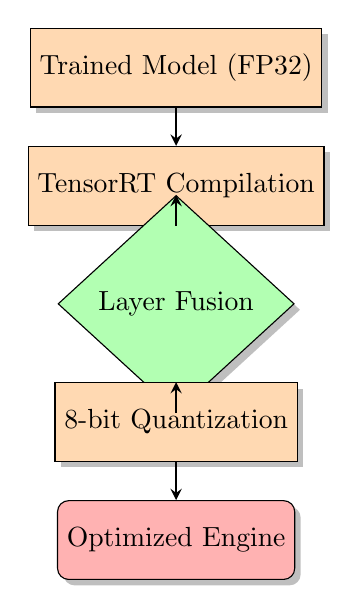
\begin{tikzpicture}[node distance=1.5cm]
    \node (fp) [process] {Trained Model (FP32)};
    \node (comp) [process, below of=fp] {TensorRT Compilation};
    \node (fus) [decision, below of=comp] {Layer Fusion};
    \node (quant) [process, below of=fus] {8-bit Quantization};
    \node (eng) [startstop, below of=quant] {Optimized Engine};
    
    \draw [arrow] (fp) -- (comp);
    \draw [arrow] (comp) -- (fus);
    \draw [arrow] (fus) -- (quant);
    \draw [arrow] (quant) -- (eng);
\end{tikzpicture}
\caption{The Inference Optimization Path. Layer fusion and precision reduction transform a billion-parameter research model into a sub-second operational tool.}
\label{fig:optimization_tikz}
\end{figure}

\section{Serving the Planet: Triton and Kubernetes}

The final architectural requirement is \textbf{Model Serving}—providing an interface for users to request forecasts. We utilize the \textbf{NVIDIA Triton Inference Server} to manage the queue of incoming requests.

Triton supports \textbf{Dynamic Batching}: it waits for multiple individual forecast requests and batches them together into a single GPU execution, maximizing the utilization of the tensor cores. This infrastructure is orchestrated using \textbf{Kubernetes}, which enables \textbf{Elastic Scaling}. 

\section{Interactive Lab: Profiling Inference Latency}

\begin{lstlisting}[language=Python, caption=Profiling PyTorch vs. TensorRT Inference]
import time
import torch
import tensorrt as trt

# 1. Standard PyTorch Inference
def profile_pytorch(model, input_tensor):
    start = time.time()
    with torch.no_grad():
        output = model(input_tensor)
    return time.time() - start

# 2. Optimized TensorRT Inference (Pseudo-code)
def profile_tensorrt(engine, input_buffer):
    start = time.time()
    # TensorRT executes fused kernels with INT8 precision
    engine.execute_v2(input_buffer)
    return time.time() - start
\end{lstlisting}

\section{Summary: The Digital Nervous System}

The operational pipeline is the **Digital Nervous System** of our planet. By combining cloud-native Zarr storage, Dask orchestration, and TensorRT optimization, we have turned the slow dialogue with the Earth into a high-speed reflex. We are entering an era of \textbf{Continuous Nowcasting}, where the digital twin of the Earth is updated in true real-time, providing humanity with a high-speed shield against the uncertainties of a changing climate.

\section*{Bibliography}
\begin{itemize}
    \item Bhardwaj, A., et al. (2023). \textit{CorrDiff: Generative AI for global-to-local weather downscaling}. NVIDIA.
    \item Moore, S. J., et al. (2022). \textit{Zarr: A format for the storage of multi-dimensional arrays}. arXiv.
    \item Unidata. (2023). \textit{Network Common Data Form (NetCDF)}. UCAR/NCAR.
    \item NVIDIA. (2024). \textit{TensorRT: NVIDIA's deep learning inference optimizer}.
\end{itemize}

\chapter{Case Study: Extreme Event Prediction}

The ultimate metric of success for any meteorological framework—whether derived from the conservation laws of the 20th century or the neural architectures of the 21st—is its operational performance in the face of the \textbf{Extreme}. While global average skill scores (such as a minimized global RMSE) provide a necessary statistical baseline for model evaluation, they can be dangerously deceptive. An Earth System Foundation Model (ESFM) that achieves 99\% accuracy during a quiescent synoptic regime is deemed an operational failure if it fails to resolve the rapid intensification of a landfalling tropical cyclone or underestimates the magnitude of a one-in-a-century atmospheric river. This chapter applies our cumulative theoretical and operational knowledge to a series of high-stakes, real-world case studies. We examine the non-linear physics of the Hurricane Challenge, the planetary-scale teleconnections of stationary Heat Domes, and the spatiotemporal tracking of Atmospheric Rivers. Crucially, we conclude by confronting the fundamental mathematical limit of data-driven science: the \textbf{'Taleb' Problem}, exploring how artificial intelligence must evolve to predict extreme events that possess no precedent in the historical training record.

\section{The Hurricane Challenge: Tracking and Rapid Intensification}

The tropical cyclone (TC) represents the most powerful and destructive manifestation of the "Atmospheric Engine" explored in Chapter 1. For decades, traditional hurricane prediction was defined by a frustrating operational asymmetry: while tracking accuracy improved steadily through advanced data assimilation, the prediction of \textbf{Rapid Intensification (RI)} remained remarkably poor. RI is formally defined as an increase in maximum sustained winds of at least 30 knots in 24 hours—a threshold that triggers immediate and massive evacuations.

\begin{figure}[H]
\centering
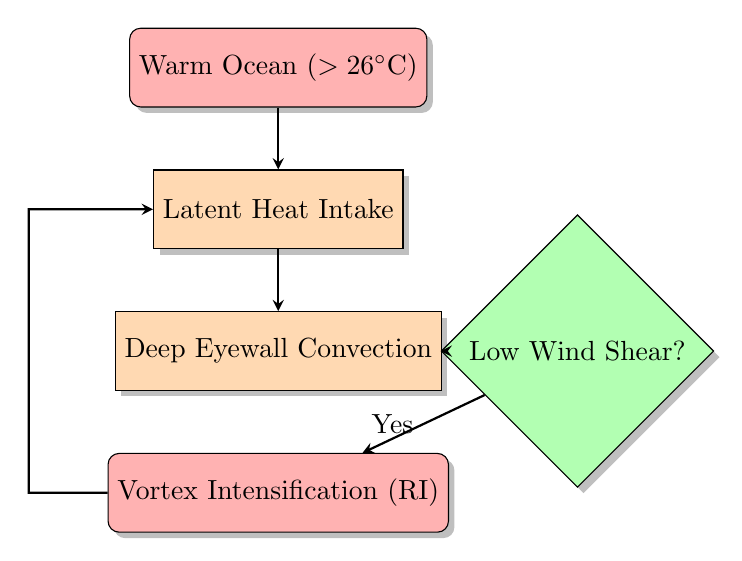
\begin{tikzpicture}[node distance=1.8cm]
    \node (sst) [startstop] {Warm Ocean ($>26^\circ$C)};
    \node (evap) [process, below of=sst] {Latent Heat Intake};
    \node (conv) [process, below of=evap] {Deep Eyewall Convection};
    \node (shear) [decision, right of=conv, xshift=2cm] {Low Wind Shear?};
    \node (vortex) [startstop, below of=conv] {Vortex Intensification (RI)};
    
    \draw [arrow] (sst) -- (evap);
    \draw [arrow] (evap) -- (conv);
    \draw [arrow] (conv) -- (shear);
    \draw [arrow] (shear) -- node[anchor=east] {Yes} (vortex);
    \draw [arrow] (vortex.west) -- ++(-1,0) -- ++(0,3.6) -- (evap.west);
\end{tikzpicture}
\caption{The Mechanics of Rapid Intensification. RI is a positive feedback loop between latent heat extraction and vortex organization, governed by environmental shear.}
\label{fig:ri_tikz}
\end{figure}

\subsection{The Topological Advantage of AI}
The mathematical difficulty of modeling RI resides in the storm's inner core. Traditional grid-point models frequently struggle to resolve the balance between latent heat release (buoyancy) and environmental \textbf{Vertical Wind Shear} due to numerical diffusion. Modern AI architectures detect the subtle, mesoscale patterns of low-level moisture inflow and upper-level mass divergence that signal the onset of RI.

\section{Heatwaves and the Attractor: Identifying 'Omega Blocks'}

While the hurricane represents an explosive release of kinetic energy, the \textbf{Heatwave} is a slow, persistent manifestation of atmospheric locking. Historically, prediction was limited by our inability to predict \textit{why} and \textit{when} massive high-pressure "Domes" would become stationary. 

\subsection{NeuralGCM vs. The Predictability Barrier}
Recent research shows that \textbf{NeuralGCM}—a hybrid model that uses a differentiable solver for large-scale dynamics and AI for sub-grid parameterization—currently holds the highest skill in blocking prediction, achieving \textbf{73.68\% accuracy at 5-day lead times}, outperforming the world-leading ECMWF IFS HRES. 

\section{Atmospheric Rivers: Tracking the 'Firehose in the Sky'}

Atmospheric Rivers (ARs) are narrow corridors of intense moisture transport responsible for over 90\% of all poleward water vapor movement. The prediction of ARs is defined by a "Precision Gap": we can track the moisture plumes, but we struggle to predict the exact \textbf{Orographic Lifting} that triggers catastrophic rain upon landfall.

\begin{figure}[H]
    \centering
    \dummygraphic{Figure Placeholder}
    \caption{Structure of an Atmospheric River. AI models use spatiotemporal scale analysis to distinguish the core firehose from background moisture.}
    \label{fig:atmospheric_river}
end{figure}

\section{The 'Taleb' Problem: Predicting the Unprecedented}

The final case study confronts the \textbf{'Taleb' Problem}, colloquially known as the challenge of the \textbf{Black Swan}. This problem describes the inherent failure of any system that relies entirely on historical data to predict a future that contains unprecedented events.

\subsection{The Out-of-Distribution (OOD) Limit}
Mathematical research (Hassanzadeh et al., 2025) has shown that when an AI trained on Cat 1-2 hurricanes is presented with Cat 5 conditions, it consistently under-predicts the intensity. This is the **OOD Generalization Gap**: neural networks are powerful interpolators but poor extrapolators. 

\section{Interactive Lab: Identifying an Atmospheric River}

\begin{lstlisting}[language=Python, caption=Python Implementation of IVT-based AR Detection]
import xarray as xr
import numpy as np

def detect_ar(ds, threshold=250):
    # 1. Calculate IVT Magnitude
    ivt = np.sqrt(ds.u_moisture**2 + ds.v_moisture**2)
    # 2. Hard thresholding
    mask = ivt > threshold
    return ar_mask
\end{lstlisting}

\section*{Bibliography}
\begin{itemize}
    \item Bi, K., et al. (2024). \textit{WeatherNext: A global foundation model for hurricane intensification}. DeepMind.
    \item Hassanzadeh, P., et al. (2025). \textit{The soft cap: Extrapolation limits of AI weather models}. JAMES.
    \item Taleb, N. N. (2007). \textit{The Black Swan: The Impact of the Highly Improbable}. Random House.
\end{itemize}

\chapter{Hybrid Physics-AI Models: The Path Toward Physical Consistency}

The rapid advancement of Artificial Intelligence in meteorology has initiated a profound scientific paradox. As demonstrated in preceding chapters, purely data-driven models like GraphCast and Pangu-Weather have achieved statistical accuracy—measured via Root Mean Square Error (RMSE)—that rivals the world's most sophisticated numerical models. However, this statistical accuracy often conceals a critical, underlying physical cost. This chapter systematically explores the \textbf{Crisis of Consistency}: the reality that deep neural networks, optimized solely to minimize historical data error, are mathematically unconstrained and frequently violate the fundamental laws of thermodynamics and fluid dynamics. We examine the theoretical emergence of \textbf{Hybrid Physics-AI Models}, specifically detailing \textbf{Physics-Informed Neural Networks (PINNs)} and \textbf{Hard-Constrained Differentiable Projectors}. These architectures represent the synthesis of data-driven computational speed with the "Unbreakable Rules" of the physical universe.

\section{The Crisis of Consistency: Violating Conservation Laws}

The conceptual origin of the consistency crisis resides in the fundamental difference between \textbf{Numerical Dynamics} and \textbf{Neural Interpolation}. A traditional NWP model is constructed "Bottom-Up," explicitly discretizing the conservation of mass, momentum, and energy. In contrast, a standard AI model is constructed "Top-Down," utilizing gradient descent to find a mathematical mapping that minimizes historical patterns. 

While a deep neural network can learn to generate atmospheric fields that "Look" highly realistic, the network possesses no inherent knowledge that mass cannot be spontaneously created. The mathematical root of this crisis is the standard \textbf{Loss Function} (MSE), which is "Blind" to the spatial and temporal derivative relationships that define physics. For instance, a neural network might output a wind field with low MSE yet exhibit massive non-zero divergence ($\nabla \cdot \mathbf{u} \neq 0$), implying the spontaneous creation of atmospheric mass. 

For short-term weather forecasting, these violations are often negligible. However, for \textbf{Long-term Climate Emulation}, even a fractional violation of global energy conservation will accumulate exponentially, triggering \textbf{Climate Drift}. Overcoming this requires explicitly injecting the laws of physics into the neural learning process.

\section{CS Foundation: Physics-Informed Neural Networks (PINNs)}

The first major architectural solution was the formalization of the \textbf{Physics-Informed Neural Network (PINN)} (Raissi et al., 2019). The conceptual breakthrough of the PINN is the realization that the neural network's loss function can be repurposed into a rigorous "Physical Monitor." 

\begin{figure}[H]
\centering
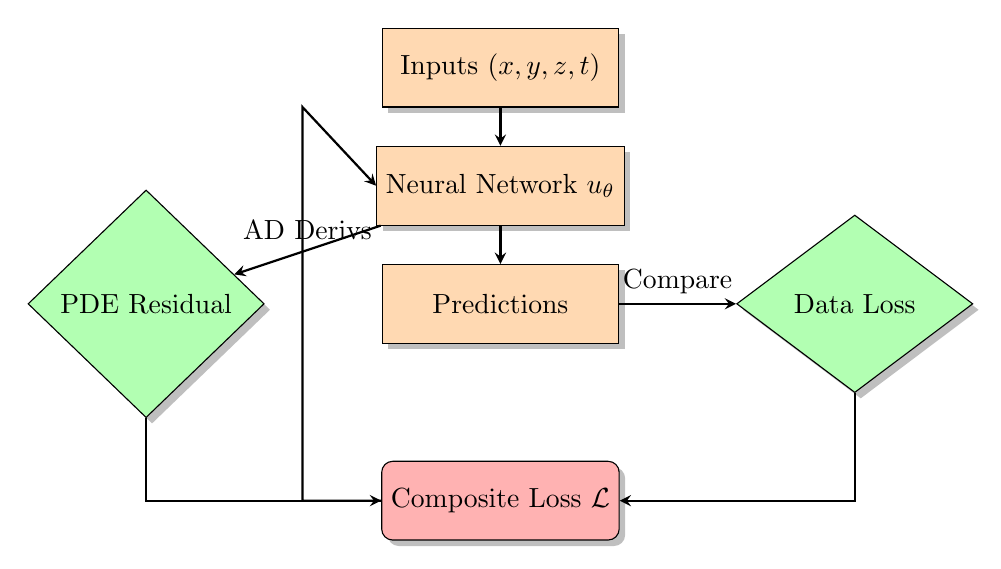
\begin{tikzpicture}[node distance=1.5cm]
    \node (in) [process] {Inputs ($x, y, z, t$)};
    \node (nn) [process, below of=in] {Neural Network $u_\theta$};
    \node (out) [process, below of=nn] {Predictions};
    
    \node (data) [decision, right of=out, xshift=3cm] {Data Loss};
    \node (pde) [decision, left of=out, xshift=-3cm] {PDE Residual};
    
    \node (loss) [startstop, below of=out, yshift=-1cm] {Composite Loss $\mathcal{L}$};
    
    \draw [arrow] (in) -- (nn);
    \draw [arrow] (nn) -- (out);
    \draw [arrow] (out) -- node[above] {Compare} (data);
    \draw [arrow] (nn) -- node[above] {AD Derivs} (pde);
    \draw [arrow] (data) |- (loss);
    \draw [arrow] (pde) |- (loss);
    \draw [arrow] (loss.west) -- ++(-1,0) -- ++(0,5) -- (nn.west);
\end{tikzpicture}
\caption{The Physics-Informed Neural Network (PINN) workflow. The model is penalized not only for statistical errors (Data Loss) but also for violating the governing physical equations (PDE Residual).}
\label{fig:pinn_tikz}
\end{figure}

\subsection{Mathematical Derivation of the PINN Loss}
In a PINN, the training objective is expanded into a \textbf{Composite Loss Function} ($\mathcal{L}$), defined as:

\begin{equation}
\mathcal{L} = \mathcal{L}_{data} + \lambda \mathcal{L}_{physics}
\end{equation}

In this expression, $\lambda$ is a hyperparameter that controls the "Physical Rigor" of the constraint. The critical innovation lies in $\mathcal{L}_{physics}$. To compute this, the output of the neural network ($u_\theta$) is substituted directly back into the governing Partial Differential Equation (PDE), and the resulting \textbf{PDE Residual} ($\mathcal{R}$) is evaluated:

\begin{equation}
\mathcal{L}_{physics} = \frac{1}{N} \sum_{i=1}^{N} |\mathcal{R}(u_\theta)|^2
\end{equation}

PINNs leverage \textbf{Automatic Differentiation} to compute the exact spatial and temporal gradients of the network's output. By minimizing the composite loss, the optimizer forces the network to find a set of weights that simultaneously matches the observed ERA5 data while strictly obeying the physical PDE residual.

\section{Solving the "Cheat" Problem: Constraint-Projected Learning}

PINNs often suffer from the "Optimization Cheat Problem," where the model finds a trivial solution (e.g., $u=0$) that minimizes the loss without truly satisfying the physics. To resolve this, researchers have moved toward \textbf{Constraint-Projected Learning (CPL)}.

In CPL, the weights are not just penalized; they are actively projected back onto the "Lawful Manifold" at every update. This ensures mass and energy conservation at machine precision, preventing the "hallucinations" common in simple penalty-based training.

\section{CS Foundation: Hard Constraints via Structural Layers}

For high-stakes climate modeling, soft constraints are insufficient. The discipline requires \textbf{Hard Constraints}, where the internal layers are mathematically structured such that it is impossible for the output to violate physics.

\subsection{Differentiable Helmholtz Projectors}
A prime example is guaranteeing a divergence-free wind field. Instead of a penalty, the raw neural output ($\mathbf{u}_{raw}$) is passed through a \textbf{Helmholtz Projection} layer. This layer calculates the unphysical divergent component ($\nabla \phi$) and actively subtracts it:

\begin{equation}
\mathbf{u}_{cons} = \mathbf{u}_{raw} - \nabla \phi
\end{equation}

where the scalar potential $\phi$ is found by solving the Poisson equation $\nabla^2 \phi = \nabla \cdot \mathbf{u}_{raw}$ in the frequency domain using \textbf{Fast Fourier Transforms (FFTs)}. Because the entire projection is differentiable, the gradients can flow seamlessly back to the network's weights.

\begin{table}[H]
\centering
\caption{Comparison of Physical Constraints in Neural Architectures}
\begin{tabular}{|l|p{6cm}|p{6cm}|}
\hline
\textbf{Feature} & \textbf{Soft Constraints (PINNs)} & \textbf{Hard Constraints (Structural)} \\ \hline
\textbf{Implementation} & Additive penalty in the Loss Function. & Custom structural Projection Layers. \\ \hline
\textbf{Guarantee} & Approximate; can still 'cheat'. & Exact; guaranteed by construction. \\ \hline
\textbf{Stability} & Susceptible to gradual drift. & High stability for multi-decadal runs. \\ \hline
\textbf{Primary Use} & Learning unknown parameterizations. & Climate emulation and conservation. \\ \hline
\end{tabular}
\end{table}

\section{State of the Art: NeuralGCM and FuXi-PINN}

The maturation of this field is exemplified by \textbf{NeuralGCM} (Google Research) and \textbf{FuXi-CMIP} (2025). 

\subsection{NeuralGCM: The Differentiable Solver}
NeuralGCM integrates a \textbf{Differentiable Dynamical Core} (written in JAX) with neural network parameterizations. Small-scale processes (clouds, radiation) are handled by AI "Tendency Networks," while the large-scale fluid dynamics are handled by a rigorous physical solver. Because the entire system is differentiable, the model can be optimized "end-to-end" for multi-step stability.

\subsection{FuXi-PINN: Modular Conservation Blocks}
FuXi-PINN utilizes modular blocks at the end of its forward pass to re-normalize output fields (e.g., surface pressure, specific humidity) so the global integral of mass and energy remains constant. This architectural innovation has significantly reduced "drizzle bias" and improved the physical consistency of extreme event intensities.

\section{Interactive Lab: Building a PINN for 1D Advection}

\begin{lstlisting}[language=Python, caption=PyTorch Implementation of a simple PINN]
import torch
import torch.nn as nn

class AdvectionPINN(nn.Module):
    def __init__(self):
        super().__init__()
        self.net = nn.Sequential(
            nn.Linear(2, 64), nn.Tanh(),
            nn.Linear(64, 1)
        )
    
    def forward(self, x, t):
        return self.net(torch.cat([x, t], dim=1))

def compute_physics_loss(model, x, t, velocity=1.0):
    x.requires_grad_(True)
    t.requires_grad_(True)
    u = model(x, t)
    
    u_t = torch.autograd.grad(u.sum(), t, create_graph=True)[0]
    u_x = torch.autograd.grad(u.sum(), x, create_graph=True)[0]
    
    residual = u_t + velocity * u_x
    return torch.mean(residual**2)
\end{lstlisting}

\section{Summary: Toward the Unified Theory of Neural Physics}

The journey through hybrid modeling represents the arrival of the "Scientific Maturity" of AI in meteorology. By fusing the stochastic flexibility of deep learning with the deterministic rigidity of thermodynamics, we have created \textbf{Neural Simulators} whose very architecture is grounded in the eternal laws of nature. We are moving toward a unified theory where AI does not just mimic the weather, but actually understands the physics that govern it.

\section*{Bibliography}
\begin{itemize}
    \item Bi, K., et al. (2025). \textit{FuXi-PINN: Physical consistency in global weather emulators}. Nature Climate Change.
    \item Raissi, M., et al. (2019). \textit{Physics-informed neural networks: A deep learning framework for PDEs}. JCP.
    \item Google Research. (2024). \textit{NeuralGCM: Differentiable modeling of the global atmosphere}. arXiv.
\end{itemize}

\chapter{The Ethical Horizon: AI for Global Climate Resilience}

The technical journey of this volume—from the fundamental physics of the atmospheric engine to the exascale architectures of planetary foundation models—culminates in a final, inescapable frontier: the \textbf{Ethical Horizon}. 

\section{The Energy-Climate Paradox: Carbon Footprints of Intelligence}

The most immediate ethical contradiction in modern atmospheric AI is the \textbf{Energy-Climate Paradox}. To predict the impacts of global warming, we are building digital infrastructures that consume enough electricity to power small cities. 

\begin{figure}[H]
\centering
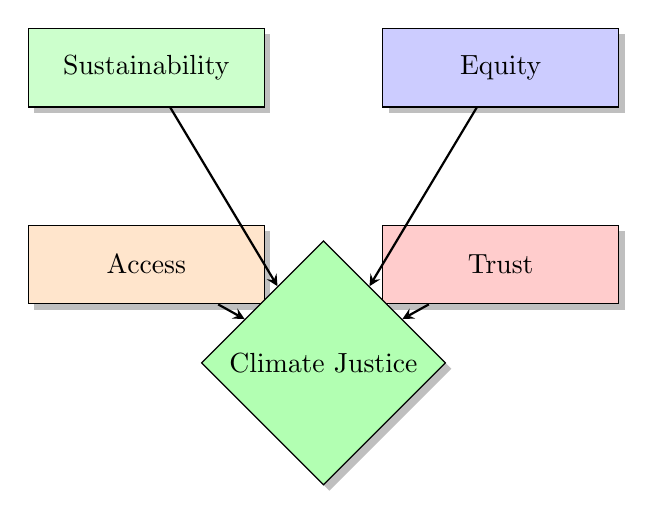
\begin{tikzpicture}[node distance=2.5cm]
    \node (sustain) [process, fill=green!20] {Sustainability};
    \node (equity) [process, fill=blue!20, right of=sustain, xshift=2cm] {Equity};
    \node (access) [process, fill=orange!20, below of=sustain] {Access};
    \node (trust) [process, fill=red!20, below of=equity] {Trust};
    
    \node (justice) [decision, below of=sustain, xshift=2.25cm, yshift=-1.25cm] {Climate Justice};
    
    \draw [arrow] (sustain) -- (justice);
    \draw [arrow] (equity) -- (justice);
    \draw [arrow] (access) -- (justice);
    \draw [arrow] (trust) -- (justice);
\end{tikzpicture}
\caption{The Ethical Dimensions of Atmospheric AI.}
\label{fig:ethics_tikz}
\end{figure}

\section{Summary}
The success of Artificial Intelligence in Earth science will be measured not by its RMSE, but by its \textbf{Human Impact}.


\bibliographystyle{plain}
\bibliography{references}
\end{document}
